
%\vspace{-5mm}
\section{The Simplified RDF Mapping Language SML}
%\todo{State that the relation between SPARQL and SPIN\url{http://spinrdf.org/}
%is similar to SML and R2RML, respectively. - Jens: not sure whether this should
% be a main point here?}

\begin{comment}
core problem is not ontological but algebraic; makes more sense to introduce a formal model and present mappings/transformations than introducing an ontology for this problem

ontology based access simplified

So far, languages for establishing RDF views on relational data have been based on XML or RDF and therefore lacked the intuitiveness of view definitions in the SQL realm.

Contributions:
\begin{itemize}
 \item formal model for RDB2RDF mappings
 \item language easier to learn than W3C
 \item less errors when writing mappings % falls sich das bei der Eval rausstellt
 \item easier debugging of mappings % besser als bei RDF-basierter Syntax z.B. keine
\end{itemize}

Analogie: Ende 90er wurde RDF/XML eingeführt da XML sehr verbreitet und deshalb als Syntax offensichtlich; analog wurde für R2RML RDF als Syntax verwendet --> in beiden Fällen angepasste Syntax übersichtlicher und leichter zu lernen
\end{comment}

% describe topic / importance
Despite the success of semantic technologies, a large share of structured knowledge still resides in relational databases.
For this reason, significant research effort has been invested by the Semantic Web community into making relational databases available as RDF.

% why: mapping languages drawbacks and advantages
Due to the strong interest in this area, several approaches and languages for mapping relational data to triples have been devised, in particular the W3C standard R2RML\footnote{\url{http://www.w3.org/TR/r2rml/}}.
While having a standard itself is of high importance, we argue that R2RML has some drawbacks on the syntactical level:
Writing RDF views in R2RML is very verbose and arguably not as intuitive as it could be.
%\todo{R4: Where is the foundation for this?
%Has a user study been created, concluding that there hasn't been an uptake of
% R2RML because of the syntax? Are the features of R2RML comparable to other languages that in the past have failed?
%Who claims this? Just the authors? (We should be able to answer this after the
% user study)}
The choice of using RDF as base syntax for R2RML has the advantage that people writing mappings can be expected to know RDF.
However, there is a significant gap between the relational database structure and the structure of the R2RML mapping specifications.
While graphical editors, such as \cite{sengupta2013editing}\cite{pinkel2014partner}, partially mitigate the problem of having to write those mapping definitions, these also have their limitations.
%First, there is a number of productive deployments where an additional component is considered a potential security risk.
%In such an environment it is also likely, that access to the host system is only provided via a text console\todo{Jens: I am not sure that this is a strong argument as you will most likely write the mapping specifications locally and then only tets and slightly refine them on the server.}, effectively hindering the utilization of a graphical frontend.
In particular, they would have to support both, the full feature set of the mapping language while still be efficient to work with and producing human readable output.
%, to cater for the scenarios previously described.
Moreover, in some environments, Web based editors in the spirit of phpmyadmin\footnote{\url{http://www.phpmyadmin.net}} may pose security risks or are not convenient, since many database and RDF experts are simply used to work on text files and textual representations of data and queries.
While they appreciate unobtrusive help, like syntax checking or code completion, a graphical user interface might impose an unfitting work flow, for example when an administrator is used to be able to perform small database related tasks via a command line interface.
In this work, we introduce the Sparqlification Mapping Language (SML) as a human friendly alternative to R2RML.
%To overcome the syntactical issues of R2RML, we introduce the SML mapping language. % in this article.
%To clarify, our intention is not to make R2RML obsolete, instead we propose an alternative syntax.
It is noteworthy, that non-RDF syntaxes for which RDF-based versions exist are commonly used the Semantic Web.
For example, while e.g. OWL ontologies can be written directly in RDF, Manchester OWL Syntax\footnote{\url{http://www.w3.org/TR/owl2-manchester-syntax/}} is a popular and concise alternative used in the primer of the OWL 2 specification itself.
As another example, while SPARQL queries in principle can be written in RDF using the SPIN SPARQL Syntax\footnote{\url{http://spinrdf.org/sp.html}}, it is uncommon to do so unless special use cases demand this.

SML is based on work towards a unified formal model for RDB2RDF mappings.
While it has equal expressiveness to R2RML, it uses a different syntactical approach:
It blends the traditional SQL \texttt{CREATE VIEW} statements with SPARQL \texttt{CONSTRUCT} queries.
Both features can be expected to be familiar to persons working on RDB2RDF data integration and combined provide a more concise syntax than R2RML.
In fact, we believe that for RDF itself, history has shown that the seemingly obvious choice of syntactically building on XML has had several drawbacks and the special purpose language Turtle meanwhile enjoys high popularity for manually crafting and editing RDF documents and Turtle 1.1 became a W3C Proposed Recommendation in 2014.
%\todo{Jörg: If not, R2RML chose ttl over xml for that very reason. Jens: I know. The point is more that RDF initially built on XML as it was popular at the same and later moved to Turtle (special purpose syntax). R2RML initially built on RDF (any serialization format) and later some people may move to SML (special purpose syntax). I think the phrasing is correct, but feel free to improve/clarify if not.}
Similarly, we believe a more intuitive special purpose RDB2RDF mapping language can provide similar benefits.

% how: briefly summarise SML
The research on the syntax of SML builds on a comparison of RDB2RDF mapping languages and a subsequently defined formal model of those languages.
Languages like R2RML and SML are syntactic instances of this formal model.
We use this model to highlight the equivalence between the languages and derive approaches for converting between them.
In particular, this implies that any processor, which can work on the W3C R2RML standard, can also use SML as input and no further implementation effort is required to use SML in combination with a number of RDB2RDF engines.
Our main argument is that SML despite its simplicity provides equal expressiveness and is, therefore, a viable alternative to R2RML.
%\todo{R4: There is no experiments or evidence that supports the claim that SML
% is a viable alternative. This one of the most important claims in the paper, but it is not supported with any evidence at all. }
% contributions
The contributions of the article are as follows:
%\vspace{-5mm}
\begin{itemize}
 \item Definition of the compact SML mapping language with equal expressiveness to R2RML
 \item Comparison of RDB2RDF mapping languages.
 \item A unified formal model of RDB2RDF mapping languages.
 \item Converters from R2RML to SML and vice versa.
 \item Syntax highlighting definition for the editor \emph{vim} and an online
 SML editor with syntax and error highlighting as a demonstrator.
 %\todo{R4: Additionally, the syntax highlighting and SML editor are clearly engineering tasks and not scientific contributions. }
 Although this component is an engineering effort, it contributed to
 the fairness of the user study in terms of providing comparable tool support
 for both R2RML and SML.
\end{itemize}
%\vspace{-5mm}

All tools, demos and the specification of the SML syntax, are available at \url{http://sml.aksw.org}.
%\todo{Jens: currently returns a 404 error}

The remainder of the article is structured as follows:
In~\autoref{sec:mapping-language-review} we review existing RDB2RDF mapping
languages. Subsequently, in~\autoref{sec:model} we present a corresponding
formal model. The SML syntax is introduced in~\autoref{sec:syntax},
whereas \autoref{sec:sml-vs-r2rml} compares it to R2RML.
In \autoref{sec:sml2r2rml} the conversion approach from SML to R2RML is described.
In \autoref{sec:eval}, we describe a user study via a public survey with 46 participants amounting to almost 16 hours of survey completion time.
Finally, we conclude this paper in~\autoref{sec:conclusion}.

%\vspace{-5mm}
\section{RDB2RDF Systems and Mapping \\ Languages Review}
\label{sec:mapping-language-review}
% Introduction

The mapping of \emph{relational databases} (RDB) to the \emph{Resource Description Framework} (RDF) is of keen interest from the inception of the \emph{Semantic Web} as exemplified in~\cite{TBL98}.
The exposition of such previously constrained data allows integration and interlinking with other data on the Web.
Based on this need, multiple tools and approaches emerged.
In an approach for fostering interoperability between those tools, the standardization of the RDB2RDF Mapping Language (R2RML) was initiated by the W3C RDB2RDF working group\footnote{\url{http://www.w3.org/2001/sw/rdb2rdf/}}.


% R2RML
R2RML is defined in \cite{r2rml} as a  mapping language for describing customized mappings of relational data into RDF.
The R2RML specification is accompanied by the Direct Mapping (DM) specification~\cite{directmapping}, describing a standard way of translating a relational database into RDF without the use of a customized mapping definition.
An R2RML mapping definition is represented in RDF using the R2RML vocabulary and serialized in the Terse RDF Triple Language (Turtle).
It can be used to either store converted relational data in an RDF dump file, expose the data as Linked Data or allow querying it via a SPARQL endpoint.
A more general overview of mapping tools for structured sources is given in~\cite{UnbehauenSeCo2012}.
Recent efforts, such as \cite{dimou2014rml}, propose extensions of R2RML for non-relational sources by adding support for the use of e.g. XPath\footnote{\url{http://www.w3.org/TR/xpath-30/}} and JSONPath expressions in the mappings.
In this work we focus on relational data.
%However, as for instance XML, these approaches are still based on creating \emph{intermediate} relations e.g. using XPath\footnote{\url{http://www.w3.org/TR/xpath-30/}} and XQuery\footnote{\url{http://www.w3.org/TR/xquery-30/}}.



% R2RML tools
With the advent of R2RML, vendors took up the standard and either modified their existing tools to additionally support R2RML or created tools fully based on the standard.
In general these tools can be categorized with regards to different dimensions, with the type of data exposition and the mode of querying the underlying database being the most distinctive.
A list of existing R2RML tools is given in~\autoref{tbl:toolcomparison}.
%Examples of Existing R2RML based tools are D2R~\cite{d2rserver}, UltraWrap~\cite{sequeda2013ultrawrap}, Ontop~\cite{rodriguez2013evaluating}, Morph~\cite{priyatna2014formalisation}, SparqlMap~\cite{unbehauen-jist-2012-sparqlmap}.
%Further tools are
These tools have in common that they all allow the exposition as SPARQL endpoint and all employ SPARQL-to-SQL translation.

The R2RML tools use the mapping definition expressed in R2RML to connect the relational data with a domain ontology.
The domain ontology describes the actual RDF data exposed and consists of standard vocabularies and custom created terms depending on the use case.
\autoref{lst:lst1} provides an example of an R2RML mapping of a simple employee table only containing IDs (\verb|EMPNO|) and names (\verb|ENAME|).
%@prefix rr: <http://www.w3.org/ns/r2rml#>.
%@prefix ex: <http://example.com/ns#>.

%\vspace{-5mm}
\begin{lstlisting}[label=lst:lst1, style=rdf,numbers=left, numberstyle=\tiny, caption=Example of an R2RML mapping.]
<#TriplesMap1>
    rr:logicalTable [ rr:tableName "EMP" ];
    rr:subjectMap [
        rr:template "http://data.example.com/employee/{EMPNO}";
        rr:class ex:Employee;
    ];
    rr:predicateObjectMap [
        rr:predicate ex:name;
        rr:objectMap [ rr:column "ENAME" ];
    ].
\end{lstlisting}

%  \todo{R4: Have the same mapping example for all the mapping languages.}

% D2RQ ML
%\vspace{-5mm}
\emph{D2RQ-ML}\footnote{\url{http://d2rq.org/d2rq-language}} is another declarative language for mapping RDB to RDF, supported by the D2R server.
As D2R is one of the most popular RDB2RDF solutions, its mapping language is also supported by other tools like UltraWrap.
The D2RQ mapping itself is an RDF document as well, usually written in Turtle syntax.
The mapping defines a virtual RDF graph that contains information from the database.
This is similar to the concept of views in SQL, except that the virtual data structure is an RDF graph instead of a virtual relational table.
The \emph{D2RQ Platform} provides SPARQL access, a Linked Data server, an RDF dump generator, a simple HTML interface, and Jena API access to D2RQ-mapped databases.
\autoref{lst:lst2} shows an example of a D2RQ mapping from a conferences table in a database to the conference class in an ontology.
%\todo{Jens: If we need more space, we could remove the location property bridge part.}

\begin{lstlisting}[label=lst:lst2, style=rdf,numbers=left, numberstyle=\tiny, caption = D2RQ map for conferences.]
map:Database1 a d2rq:Database;
    d2rq:jdbcDSN "jdbc:mysql://localhost/iswc";
    d2rq:jdbcDriver "com.mysql.jdbc.Driver";
    d2rq:username "user";
    d2rq:password "password";
    .
map:Conference a d2rq:ClassMap;
    d2rq:dataStorage map:Database1.
    d2rq:class :Conference;
    d2rq:uriPattern "http://conferences.org/comp/confno@@Conferences.ConfID@@";
    .
map:eventTitle a d2rq:PropertyBridge;
    d2rq:belongsToClassMap map:Conference;
    d2rq:property :eventTitle;
    d2rq:column "Conferences.Name";
    d2rq:datatype xsd:string;
        .
\end{lstlisting}
%	map:location a d2rq:PropertyBridge;
%	    d2rq:belongsToClassMap map:Conference;
%	    d2rq:property :location;
%	    d2rq:column "Conferences.Location";
%	    d2rq:datatype xsd:string;
%	    .

  Generally speaking, D2RQ-ML is close to R2RML with some notable distinctions.
D2RQ-ML includes the database connection information in the mapping file and uses different constructs to express joins between tables.

% tool specific ML
Another notable approach is utilized in the ontop\cite{ontop} platform by the
\emph{Knowledge Representation meets Databases (KRDB)}\footnote{\url{http://www.inf.unibz.it/krdb/}} research group.
Ontop supports mapping definitions in its own language and R2RML.
Quest, the SPARQL engine/reasoner in ontop, implements query rewriting techniques that translate SPARQL into SQL.
\autoref{lst:lst3} shows an example from the ontop
documentation\footnote{\url{https://github.com/ontop/ontop/wiki/ontopOBDAModel}}.
%\footnote{\url{https://github.com/ontop/ontop/wiki/ObdalibObdaFile}}.

%a table from \emph{IMDB\footnote{\url{http://www.imdb.com/}}} to RDF using
% \emph{Music Ontology}(MO)\footnote{\url{http://musicontology.com/}}.

\begin{lstlisting}[label=lst:lst3, style=sparql,numbers=left, numberstyle=\tiny, caption = Example of the Ontop mapping language]
[MappingDeclaration] @collection [[
  mappingId     Book collection
  target        :BID_{id} a :Book .
  source        SELECT id FROM books
]]
\end{lstlisting}

%  \begin{lstlisting}[label=lst:lst2, style=sparql,numbers=left,
  % numberstyle=\tiny, caption = Example of the Ontop mapping language] Source (SQL Query):
%	  SELECT id, title FROM title
%	Target(Triples Template):
%	  <"&:;title/{$id}"> a mo:Movie; mo:title ?title .
  %\end{lstlisting}
% Virtuoso RDF views
\emph{Virtuoso RDF Views}~\cite{virtuosoRdfViews} is another tool specific mapping language.
It is part of OpenLink's Virtuoso Universal Server\footnote{\url{http://virtuoso.openlinksw.com/}}.
Virtuoso RDF Views provide a declarative Meta Schema Language for mapping of SQL data to RDF ontologies and preceded Virtuoso's R2RML support.
%Virtuoso RDF views mapping is dynamic; in a science that changes to the underlying data are reflected immediately in the RDF views.
The corresponding mappings are dynamic, such that changes to the underlying data are reflected immediately in the RDF views.
OpenLink Virtuoso Universal Server includes SPARQL support and an RDF data store tightly integrated with its relational storage engine.
An example of a Virtuoso RDF View definition is given in \autoref{lst:lst4}.

%prefix rdf: <http://www.w3.org/1999/02/22-rdf-syntax-ns#>
%prefix prd: <http://localhost:8890/rdfv_demo/schemas/product#>

\begin{lstlisting}[label=lst:lst4, style=rdf,numbers=left, numberstyle=\tiny, caption = Virtuoso RDF views example]
graph <http://localhost/testdata/products#>
subject prd:product_iri(PRODUCT.PRODUCT_ID)
predicate rdf:type
object prd:Product
  \end{lstlisting}

%Graphical based ML

Besides the textual mapping languages, there are also tools providing a graphical representation of the mapping.
The \emph{Asio Semantic Web bridge} SBRD\footnote{\url{http://bbn.com/technology/knowledge/asio_sbrd}} or the more recent R2RML editor presented in~\cite{r2rmleditor} fall into this category.
SBRD utilizes \emph{Snoggle}\footnote{\url{http://bbn.com/technology/knowledge/snoggle}} for mapping from RDB to RDF.
\emph{Snoggle} is a graphical ontology mapper based on the \emph{Semantic Web Rule Language} (SWRL)\footnote{\url{http://www.w3.org/Submission/SWRL/}}.
It allows users to draw ontologies and then create mappings between them on a graphical canvas.
This mapping is then translated into SWRL/RDF or SWRL/XML.
%An example of the \emph{Snoggle} visual mapper in provided in
%\autoref{fig:snoggle}

An overview of the introduced RDB2RDF solutions is given in \autoref{tbl:toolcomparison}.
% \begin{figure}[tbh]
% \centering
% 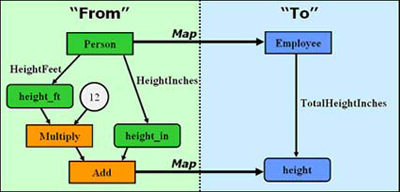
\includegraphics{Snoggle.jpg}
% \caption{Example of the graphical mapping of \emph{Snoggle} based on the Semantic Web Rule Language (SWRL)\todo[inline]{Replace by high resolution figure!}}
% \label{fig:snoggleXX}
% \end{figure}

%SNOGGLE WAS HERE


%% \begin{table*}[ht]
%%     \centering
%%     \caption{Comparison between different mapping tools}
%%     \small
%%     \begin{tabular}{@{}p{2.8cm}   p{2.1cm}   p{2.1cm}  p{2.1cm}  p{2.1cm}  p{2.1cm} @{}}
%%     \toprule
%%
%%     \textbf{Features/Tool} 	& \textbf{Ontop}	& \textbf{Revelytix Spyder}	& \textbf{Asio SBRD} 	& \textbf{Virtuoso RDF Views} 	& \textbf{D2RQ Platform}\\
%%     \midrule
%%
%%     Mapping language	& Own language	\& R2RML  	& R2RML				& Graphical 		& Own language \& R2RML 			& D2RQ-ML\\
%%     SPARQL support 		& 1.0  			& 1.1 				& × 			& 1.1 				& 1.1\\
%%     License		& Free for non-profit purposes& Free			& Commercial	 	& Free 				& Free\\
%%     Support		& Free 			& With fees 			& Commercial 		& Free 				& Free\\
%% %    DBMS Support 	& Almost all		& Almost all			& Almost all		& Virtuoso			& Almost all\\
%% % not differentiated enough
%%     \bottomrule
%%     \end{tabular}
%%     \label{tbl:toolcomparison}
%% \end{table*}
%% for non-profit purposes

\begin{table*}[ht]
    \centering
    \small
% {\textwidth}
%     \begin{tabular}{@{}p{90pt}p{60pt}p{50pt}p{80pt}p{50pt}@{}}
% \begin{tabularx}{\textwidth}{@{}XXXXXXXXXXXX@{}}
      \begin{tabularx}{\textwidth}{@{}XXXXX@{}}
      \toprule
      \textbf{Tool/Features}  & \textbf{Mapping language}   & \textbf{SPARQL Version} & \textbf{License}  & \textbf{Support}  \\
      \midrule
      Ontop~\cite{rodriguez2013evaluating}                  & Own language \& R2RML       & \centering 1.0          & Free              & Free              \\
      Revelytix Spyder        & R2RML                       & \centering 1.1          & Free              & With fees         \\
      Asio SBRD               & Graphical                   & \centering ---          & Commercial        & Commercial        \\
      Virtuoso RDF Views~\cite{virtuosoRdfViews}      & Own language \& R2RML       & \centering 1.1          & Free              & Free              \\
      D2RQ Platform~\cite{d2rserver}           & D2RQ-ML                     & \centering 1.1          & Free              & Free              \\
      Morph~\cite{priyatna2014formalisation}                   & R2RML                       & \centering 1.0          & Free              & Free              \\
      Ultrawrap~\cite{sequeda2013ultrawrap}               & R2RML                       & \centering 1.0          & Commercial        & Commercial        \\
      SparqlMap~\cite{unbehauen-jist-2012-sparqlmap}        & R2RML                       & \centering 1.0          & Free              & Commercial        \\
      Sparqlify               & R2RML \& SML                & \centering 1.0          & Free              & Free              \\
      \bottomrule
%     \end{tabular}
      \end{tabularx}
    \caption{Comparison between different mapping tools and languages.}
    \label{tbl:toolcomparison}
\end{table*}
%Sparqlify~\footnote{\url{https://github.com/AKSW/Sparqlify}}, Revelytix Spyder~\footnote{\url{http://www.revelytix.com/?q=content/spyder}}
%\tablefootnote{\url{http://www.revelytix.com/?q=content/spyder}}

%~\footnote{\url{http://www.revelytix.com/?q=content/spyder}}

%\todo{R3: Table 1 is a very general comparison. I would expect a comparison on
% the constructs and expressiveness of the different languages.}

%\section{Tabular Data to RDF Transformation}
% \section{A Formal Model for RDB2RDF Mappings}
%\vspace{-5mm}
\section{Towards a Unified Formal Model for RDB2RDF Mappings}
%\todo{first version Claus, Jens proof read}
\label{sec:model}

In this section, we outline a formal approach for mapping tabular data to RDF.
For this purpose, we first briefly summarize fundamental concepts of the RDF data model.
It should be noted, that we assume that RDF is generated by
\emph{row-wise} processing of the underlying relational data.
Both R2RML and SML build on this assumption.
Also, without loss of generality, we only consider quads rather than triples in the formalization.
The reason is, that we can view any generated triple as being labeled with the URI of the graph it belongs to.

\paragraph{Preliminaries}
\label{sec:transformation-preliminaries}
Let the RDF primitives be: $\mathcal{U}$ the set of URIs, $\mathcal{B}$ the set
of blank nodes, $\mathcal{L}$ the set of literals and $\mathcal{V}$ the set of
variables. Further:
\begin{itemize}
% \item $\mathcal{U}$ is the set of URIs
% \item $\mathcal{B}$ is the set of all blank nodes
% \item $\mathcal{L}$ is the set of all literals
% \item $\mathcal{V}$ is the set of all variables
 \item $\mathcal{T}$ is the set of all \emph{RDF term}s, defined as
  $\mathcal{U} \cup \mathcal{B} \cup \mathcal{L}$.
\end{itemize}

Furthermore, we make use of the following notions:
\begin{itemize}
  \item $\mathcal{J}$ is the joint set of RDF terms and variables, defined as $\mathcal{T} \cup \mathcal{V}$.
  \item $\mathcal{Q}$ is the set of all \emph{quads}, defined as $\mathcal{J} \times \mathcal{J} \times \mathcal{J} \times \mathcal{J}$.
  \item A \emph{quad pattern} $Q$ is a finite, possibly empty, set of quads, defined as $Q
  \subset \mathcal{Q}$
%  \todo{probably we should write "finite set" or $Q \subseteq \mathcal{Q}$?}
  \item $\mathcal{R}$ is the set of all quad patterns, thus the powerset of $\mathcal{Q}$, denoted by $\mathcal{P}(\mathcal{Q})$
  \item A \emph{quad} $q$ is defined as $q \in \mathcal{Q}$.
  \item $vars(Q)$ is the set of variables appearing in $Q$.
  \item A \emph{ground quad (pattern)} is a variable free quad (pattern).
\end{itemize}
%\footnote{For clarification: there is a small inconsistency in the terminology: A triple pattern is an element, whereas a quad pattern is a set.}

%Finally, we introduce our notion of a \emph{logical table} $L$, which we define
%as a set of partial functions that map attribute names to attribute values.
Finally, we introduce our notion of a \emph{relation instance} (short: relation) $L$, which, for convenience, we
define as a \emph{set of partial functions} that map attribute names to
attribute values.
It is noteworthy, that R2RML defines an entity referred to as \emph{logical
table}. Instances of this entity possess an
\emph{effective SQL
query}\urlfn{http://www.w3.org/TR/r2rml/\#dfn-effective-sql-query} which can be evaluated over an instance
of a database schema in order to obtain a relation.


%Finally, for ease of discussion, we introduce the function $\sigma$ that
%transforms all rows of a canonical table $C$ into a \emph{logical table} $L$,
% which is a set of corresponding partial functions from headings to data, i.e. a table
%\[
%((id, name), \{(1, Anne), (2, John) \})
%\]
%is transformed to:
%\\[
%\{ \{(id, 1), (name, Anne) \}, \{(id, 2), (name, John) \} \}
%\]

%Let $\mathcal{C}$ and $\mathcal{L}$ be the set of all canonical and logical
%tables, respectively.
%Note, that this representation is analogous to the one defined for SPARQL result sets\todo{ref to sparql spec}.
%\[
%\mathit{\sigma}: \mathcal{C} \rightarrow \mathcal{L} \newline
%\]
%\[
%\sigma(C): = \left \{ \bigcup_{1 \leq i \leq |C.H|} \left \{ (C.H_i, d_i)
% \right \} \Bigg\vert d \in C.D  \right \}
%\]

\paragraph{Generating RDF from relations}
Based on the previously introduced primitives, we are now able to formally
capture the nature of RDF mapping approaches for relational data.
%\todo{maybe
%replace tabular by relational}

A relational data to RDF (\emph{R2R}) mapping $m$ is a four-tuple $(N, P, L, f)$:
\begin{itemize}
  \item {$N$} is the \emph{name} of a view.
  \item {$P$} is a \emph{quad pattern}
%  \todo{Would it make sense to use $Q$ here as this is the latter used for quad patterns? (would need replacement further down as well)}
   which acts as the \emph{template} for the construction of triples and
   relating them to named graphs. The template is instantiated once for each row
   of the relation.
%  The use of quads enables one to map tabular data into distinct named graphs.
%  We use the notation $vars(P)$ for referring to the set of SPARQL variables
%  used in the template.
  \item {$L$} is a relation to be converted to RDF.
  \item {$f$} is a mapping with signature $L \rightarrow \left( \mathcal{V} \rightarrow \mathcal{T} \right)$:
  $f$ yields for each element of the relation $L$ a partial function that binds
  the variables of the template $P$ to RDF terms in $\mathcal{T}$.
  Note that it is not required for variables of $P$ to be bound, which enables the support NULL values in the source data.
\end{itemize}
An R2R mapping is valid, if its \emph{evaluation} yields an
\emph{RDF dataset}, as defined in the SPARQL
secification\urlfn{http://www.w3.org/TR/sparql11-query/\#rdfDataset}.
%\todo{Do we need to clarify what "conforms to" means here? Or can we just say
%that the evaluation returns a dataset (as defined in the SPARQL spec)?}

Given a quad pattern $Q \subset \mathcal{Q}$ and a partial function $a: \mathcal{V} \rightarrow \mathcal{T}$, we define the substitution operator
\[
\mathit{\rho_{[a]}}: \mathcal{R} \rightarrow \mathcal{R}
\]
$\rho_{[a]}(Q)$ yields a new ground quad pattern $Q'$ with all variables replaced in accordance with $a$. Any quads of $Q$ with unbound variables
in $a$ are omitted in $Q'$.
%\rho{a / b}(P) which replaces all variables in a quad pattern
%$
%\rho_{[a / b]} \left(R \right) := \left(
%    \rho_{[a / b]} \left( R_{D} \right),
%    \rho_{[a / b]} \left( R_{l} \right)
%\right)
%$

An evaluation of a mapping $m$ proceeds by
passing each row of $L$ as an argument to $f$,
thereby obtaining the bindings for $vars(P)$,
which are used to instantiate the template $P$
%\todo{"concrete quads" is undefined - just "quads"?}
for finally creating ground quads. Let $\mathcal{M}$ be the set of all mappings, then a function $\mathit{eval}: \mathcal{M} \rightarrow \mathcal{R}$ can be defined as:
%\[
%\mathit{eval}: \mathcal{M} \rightarrow \mathcal{R}
%\]
%\[
%eval(m) = \bigcup_{l \in m.L} \left\{ \rho_{[m.f(l)]}(m.P) \right\}
%\]

\[
eval(m) = \bigcup_{l \in L} \left\{ \rho_{[f(l)]}(P) \right\} \quad \text{ with } m = (N,P,L,f)
\]
%\todo{alternative suggestion without the dot notation}

What remains is to define a representation of the function $f$ in terms of
expressions. We refer to such a set of expressions as a \emph{variable definition}.
An analysis of the mapping languages revealed, that there is a small set
of essential operations for RDB-to-RDF mappings, for which we devised an
Extended Backus–Naur Form (EBNF) of an expression grammar as shown in
\autoref{lst:vardef} and explained as follows.

In a first step, we need to be able to construct RDF terms from the
underlying relation, hence we introduce the
\emph{rdf-term-ctor-expr}\footnote{We use \emph{ctor} as abbreviation for \emph{constructor}} production.
Note that our \texttt{plainLiteral} and \texttt{typedLiteral} functions
roughly correspond to the functions\texttt{STRDT} and \texttt{STRLANG} of the SPARQL standard,
although in SML arguments may be of types other than string, such as when mapping a column of type real to a corresponding typed literal.
Yet, in the future aliases may be introduced to SML for better alignment with existing SPARQL features.

%, and
%any variable definition that yields RDF terms would be valid for $f$.
An analysis of the mapping languages revealed, that there is a small set
of essential operations for RDB-to-RDF mappings,
namely \emph{concat}, \emph{str} and \emph{urlEncode} and
\emph{percentEncode}\footnote{\url{http://tools.ietf.org/html/rfc3986}}.
%Furthermore, for converting values from the database into IRI-safe values,
%there is also
% \emph{percentEncode}\.
These function symbols are usually used for the construction of URIs and
IRIs from values of the underlying relation: The function symbol
\emph{concat} may be used to prepend a prefix IRI to one or more ID columns.
The function symbol \emph{str} corresponds to an implicit conversion and
therefore usually does not have to be stated explicitly as it can be implied.
It is needed to preserve type consistency:
For instance, \emph{concat} is only defined for string arguments.
Therefore, \emph{concat}('http://ex.org/', 1) would yield a type error without
the prior conversion of the second argument to string.
%Another example is, that
%when creating plain l


%\todo{Can we say, e.g., that those are supported by all mapping languages
% analysed in the previous section? This part should not sound SML specific, so we might mention a reason why there are exactly those 3 (even it is obvious for you).}

Note, that although these functions could
be applied in the underlying RDBMS, support at the mapping level opens
possibilities for basic optimizations without the need to parse the involved
SQL.

%An Extended Backus–Naur Form (EBNF) of the expression grammar
%\todo{The switch from mathematical notation to EBNF might be seen as going from
% the high level model to a specific syntax already, which is a bit dangerous in this section.}
%is shown in \ref{lst:vardef}. It is noteworthy, that this grammar captures the
%essence of the constructs that R2RML introduces for the purpose of constructing
%a set of RDF terms from a row of a logical table.

\begin{lstlisting}[caption=EBNF for variable definition expressions, label=lst:vardef]
varDefinition = (var '=' rdf-term-ctor-expr)* ;

rdf-term-ctor-expr
    = bNode '(' expr ')'
    | uri '(' expr ')'
    | plainLiteral '(' expr (',' expr)? ')'
    | typedLiteral '(' expr ',' expr ')'
    ;

expr-list
    = (expr (',' expr)*)?
    ;

expr
    = var     // Denotes a reference to a column
    | str '(' expr ')'
    | concat '(' expr-list ')'
    | urlEncode '(' expr ')'
    ;
\end{lstlisting}

Example:
Assume a given relation holding the label of a product:
\[
\left\{ \left\{ (\text{id}, \text{1}), (\text{label}, \text{``Coke''}) \right\}, \ldots \right\}
\]
Assume that we aim to obtain the following assignment from variables
to RDF terms:
\[
\left\{ \left\{ (?s, \text{<http://ex.org/1>}), (?l, \text{``Coke''@en}) \right\}, \ldots
\right\}
\]

Then a definition of $f$ as
\begin{multline}
f: [\{ ?s = \text{uri}(\text{concat}(\text{'http://ex.org/'}, \text{str}(?id))), \\
      ?l = \text{plainLiteral}(?label, \text{'en'})
\}]
\end{multline}
would yield the desired output.

%\[
%f({{(id, 1)}}) = {{(?s, <http://ex.org/1>)}}
%\]

%It is noteworthy, that in practice
%\todo{Maybe say something about datatypes}
%\vspace{-5mm}
\section{SML Syntax}
\label{sec:syntax}

In this section, we give an introduction to the SML syntax.
%This is followed by a detailed formalization of the SPARQL-SQL rewriting.
%The innovation of SML's view definition syntax is to blend the concepts of
% traditional SQL \emph{Create View} statements with those of SPARQL \emph{Construct} queries.
%The mapping language is therefore composed of features that a person working on
% RDB-RDF data integration is likely to be already familiar with.
% Jens => erwähne ich jetzt später
% For this reason, we expect SML to be easier to learn and use than other mapping approaches (which define a completely new mapping language).
%imitations and future work of the language are discussed in
% \autoref{sec:conclusion}.

The left hand side of \autoref{fig:sparqlify-ml-r2rml} shows an example of SML,
whose syntactic constituents are explained as follows.

% juxtaposes the syntactic
%outline of the language with an example.

%\begin{figure}[htb]
%\centering
%\begin{tabular}{lll}
%\toprule
%\emph{Outline} & \emph{Example}  \\
%\midrule
%
%\begin{minipage}{5cm}
%\begin{scriptsize}
%\begin{verbatim}
%CREATE VIEW <name> AS
%  Construct {
%    <GraphConstructTriples>
%  }
%  WITH
%    <VariableDefinitions>
%  CONSTRAIN
%    <ConstraintDeclarations>
%  FROM
%    <LogicalTable>
%\end{verbatim}
%\end{scriptsize}
%\end{minipage}

%&


%\begin{minipage}{5cm}
%\begin{scriptsize}
%\begin{verbatim}
%CREATE VIEW hotels AS
%  CONSTRUCT {
%    ?s a ex:Hotel .
%    ?s rdfs:label ?l .
%    ?s ex:vacancy ?v .
%  }
%  WITH
%    ?s = uri(?website)
%    ?l = plainLiteral(?name, 'en')
%    ?v = typedLiteral(?vacancy,
%              xsd:boolean)
%  CONSTRAIN
%    ?s prefix "http://ex.org/"
%  FROM
%    [[SELECT website, name, vacancy
%      FROM hotels]]
%\end{verbatim}
%\end{scriptsize}
%\end{minipage}
%
%\end{tabular}
%\caption{SML view definition syntax.}
%\label{fig:sparqlify-ml}
%\end{figure}



Recall that in the previous~\autoref{sec:transformation-preliminaries} we
formally defined an R2R view as a four-tuple $(N, P, L, f)$.
The core syntax of an SML view definition comprises four parts that correspond
directly to the formal definition. Additionally, SML features
an optional \emph{constraint} component for improving query performance.
%a \emph{constraint} component, that turned out to be useful in pratice.
An SML view definition is composed of the following parts:
\begin{itemize}
  \item The \emph{name} of the view. This corresponds to an element of the
  set $N$.

  \item A \emph{construct} clause, which consists of triple patterns
  which can be optionally associated with a specific named graph by
  surrounding
  them with \texttt{GRAPH }$G${ \{ \ldots \}}, where $G$ can be a variable name
  or an IRI.
  %The syntax is therefore a slight extension of the \emph{ConstructTemplate}
  % production rule\footnote{\url{http://w3.org/TR/rdf-sparql-query/\#sparqlGrammar}} of SPARQL.
  Hence, the syntax is equivalent to the \emph{quads} production rule of the
  SPARQL 1.1 standard\footnote{\url{http://www.w3.org/TR/sparql11-query/\#rQuads}}.
  This corresponds to an element of $P$.

  \item A \emph{FROM} clause, where a reference to a \emph{logical table} can be specified.
  As in R2RML, this can be either an SQL SELECT statement, the name of a
  physical table or the name of a view.
  The former needs to be escaped in triple double-quotes, i.e. \texttt{"""SELECT \ldots"""}.
  The execution of a logical table's effective SQL query over an SQL connection
  yields a result set which formally corresponds to $L$.

  \item The \emph{variable definition clause} acts as the bridge between the RDF
  and SQL data models, and is used to specify the creation of RDF terms from
  rows of the relation.
  It consists of a set of \emph{variable definition statements} of the
  form \emph{?var = rdf-term-ctor($expr_0$, \ldots, $expr_n$)}, and should
  at least support the grammar defined in \ref{lst:vardef}.

%
%  \begin{itemize}
%    \item $\mathit{termctor}$ refers to the RDF term constructor, which can be
    % \texttt{bNode}, \texttt{uri}, \texttt{plainLiteral}, or \texttt{typedLiteral}. %It is discussed in more details in\todo{reference - I want to say something about its datatypes}.
%    \item $expr_i$ refers to expressions over sets of SQL column references of
    % the logical table and constants.
%			Syntactically, the currently supported operators in variable definition
            % expressions are:
%			\texttt{concat}, \texttt{urlEncode} and \te.%Note that our
            %formalization arbitrary SQL expressions are allowed.
%    \item $var$ is a SPARQL variable being defined, which should be referenced
    % from the construct clause.
            %Note that these expressions are treated specially by the Sparqlify engine's optimizer.
            %Sparqlify does not try to understand the SQL, for this reason expressions
            %Note that expressions stated in the projections of SQL queries are not subject to query optimization by Sparqlify.
%  \end{itemize}

  \item Finally, there is a \emph{CONSTRAINT} clause for specifying
  contstraints about variables on the RDF level. As such, it has no direct
  influence on the virtual RDF relation, but rather on query performance.
  The example in \autoref{fig:sparqlify-ml-r2rml} shows, that
  solely based on the definition of $?s = uri(?website)$ we have no information
  about the set of URIs being created. Specifying such a type of constraints
  enables SPARQL-to-SQL rewriters, for instance, to prune joins whose join
  condition equates variables with disjoint sets of prefixes. Syntactically, up
  to now only stating prefix constraints is supported.
   %can be explicitely
  %specified.
  %Internally, however, constraints are used to restrict predicates to URIs or
  % subjects to blank nodes and URIs.
\end{itemize}

%It is noteworthy that the `variables' used as arguments of the term
%constructors are column references to the relation and as such carry a SQL
%datatype.
%This means that RDB2RDF mappings need to be datatype aware.



%\begin{definition}[Correctness and Completeness of Rewrites]
%RDF-Relation = materialize(Views, Database)

%DumpQueryResultSet = Execute(RDF-Relation, SparqlQuery)

%Rewrite(SparqlQuery, Views) returns (SqlQuery, Map)
%ViewQueryResultSet = Map(Execute(Database, SqlQuery))

%Correct: ViewQueryResultSet subset DumpQueryResultSet
%Complete: ViewQueryResultSet superset DumpQueryResultSet


%TODO Place datatypes into the view definition? I guess this makes most sense,
%because then we do not have to carry the database around.

%TODO How to show that we are preserving this for most of the time?
%\end{definition}



%\vspace{-5mm}
\section{Comparison of SML with R2RML}
\label{sec:sml-vs-r2rml}
%--\todo{R3: section 5 is titled "Comparison of SML with R2RML" whereas the contribution of the paper is supposed to be  the converters of the languages - both ways. If this is the case, then the section title should be changed and the mappings of SML to R2RML and vice versa should be defined or at least a Table of the correspondence between the constructors of both languages should be presented, it is only presented for term constructors to term maps.}
In this section, we summarize essential features of R2RML and explain how
they relate to those of SML.
R2RML mappings are expressed as RDF graphs for which R2RML by convention uses
Turtle serialization. The fundamental class is \texttt{rr:TriplesMap}, whose
instances are specifications of the triples to generate from an underlying
logical table.
As such, an instance of a TriplesMap corresponds to an SML view definition.
In the following, we explain the most important attributes that TriplesMaps
may have, and compare them to SML.
\autoref{fig:sparqlify-ml-r2rml} shows a side-by-side
comparison of the mapping languages for a specific example.
Both syntactic formats can be converted to each other.

\begin{figure*}[t]
\centering
\begin{tabular}{@{}ll@{}}
\toprule
\emph{SML} & \emph{R2RML}  \\
\midrule
  \begin{minipage}{0.38\linewidth}
    \begin{scriptsize}
\begin{verbatim}
Prefix rdfs: <http://www.w3.org/2000/01/rdf-schema#>
Prefix xsd: <http://www.w3.org/2001/XMLSchema#>
Prefix ex: <http://ex.org/>

Create View hotels As
  Construct {
    ?s a ex:Hotel ;
      rdfs:label ?l ;
      ex:vacancy ?v
  }
  With
    ?s = uri(?website)
    ?l = plainLiteral(?name,'en')
    ?v = typedLiteral(?vacancy,
              xsd:boolean)
  Constrain
    ?s prefix "http://ex.org/"
  From
    """SELECT website, name,
      vacancy FROM hotels"""
\end{verbatim}
    \end{scriptsize}
  \end{minipage}
  &
  \begin{minipage}{0.60\linewidth}
\begin{scriptsize}
\begin{verbatim}
@prefix rdfs: <http://www.w3.org/2000/01/rdf-schema#> .
@prefix xsd: <http://www.w3.org/2001/XMLSchema#> .
@prefix ex: <http://ex.org/> .

<HotelTriplesMap>
  rr:logicalTable [ rr:sqlQuery
  """SELECT website, name,
  vacancy  FROM hotels""" ];

  rr:subjectMap [
    rr:column "website";
    rr:class ex:Hotel
  ];
  rr:predicateObjectMap [
    rr:predicate rdfs:label;
    rr:objectMap
      [ rr:column "name";
        rr:language "en"];
  ];
  rr:predicateObjectMap [
    rr:predicate ex:vacancy;
    rr:objectMap
      [ rr:column "vacancy";
        rr:datatype
          xsd:boolean ];
  ].
  \end{verbatim}
\end{scriptsize}

\end{minipage}
\\\bottomrule
\end{tabular}
%\vspace{-5pt}
\caption{A simple view in SML and R2RML.}
\label{fig:sparqlify-ml-r2rml}
\end{figure*}%\todo{The rdf:type predicateObjectMap is missing in the `A simple view in SML and R2RML' figure. Maybe use ldots to show that it is left out intentionally}

%The following paragraphs
%we base our discussion on the paragraphs as they
%appear in the R2RML standard.

% is an RDF vocabulary for expressing
%RDB2RDF mappings
%, originally inspired by the D2RQ mapping vocabulary.
%R2RML and SML are both very recent and
%independent efforts whereas the latter has since then evolved into a W3C
% Proposed Recommendation\footnote{\url{http://www.w3.org/TR/r2rml/}}.
%The core concepts of R2RML have semantically equivalent counterparts in
%SML and vice versa.

% However, users can benefit from SML for
%two reasons:
%\begin{itemize}
%  \item We expect SML to be easier to learn and use for typical users than other mapping approaches, including R2RML, since it composes SPARQL and SQL constructs with few additional constructs.
%  \item For typical RDB2RDF mapping authors, we expect SML to be easier to
  % learn and use than other mapping approaches, including R2RML, since it composes SPARQL and SQL constructs with few additional syntactical elements.
%  \item The SML syntax is more compact due to less syntactic noise created by
  % using an XML based format.
%  \item The syntax and the corresponding formal model are conceptually very close.
%\end{itemize}

%A potential further advantage is that the syntax and the underlying formal
% model are conceptually closer in SML than in R2RML.
%
%RDF generation is performed in both cases by applying on logical tables
% row-wise mapping instructions.
% their RDF terms are constructed in R2RML and outline their corresponding SML expressions.

%\vspace{-5mm}
\paragraph{Defining Logical Tables}
R2RML defines the predicate \texttt{rr:logicalTable} to relate a TriplesMap to a
logical table. The object of this predicate must be a resource that is further
described using \texttt{rr:tableName} or \texttt{rr:sqlQuery}.
A TriplesMap must have exactly one logical table.
In SML, the \emph{FROM} clause serves the same purpose.
\autoref{tbl:from-clause} compares how to state a logical table in
R2RML and SML.
%Note that in SML it is valid to omit the FORM and WITH clause, if the template
%only contains concrete quads. A common use case is specifying parts of the
%vocabulary, such as domain and range.

%Note that in SML
%it is valid to omit the FROM and WITH clause, if the template only holds
%concrete quads. Technically, it is equivalent to using [[SELECT 1]]

\begin{table}[!h]
\centering
\begin{scriptsize}
\begin{tabular}{ll}
\toprule
rr:tableName "person"       & \ldots From person \\
rr:tableName "SCOTT.DEPT"   & \ldots From "SCOTT.DEPT" \\
rr:sqlQuery """SELECT \ldots""" & \ldots From """SELECT \ldots""" \\
%\midrule
\bottomrule
\end{tabular}
\end{scriptsize}
\caption{Comparison of attributes of rr:logicalTable with SML's FROM clause.}
\label{tbl:from-clause}
\end{table}

% omitted due to space

%A minor difference is that R2RML additionally supports stating the dialect of
%an SQL query using the \texttt{rr:sqlVersion} property, which at present, has no counterpart in SML.
%This flag could be used to hint a mapping processors to pick a specific SQL parser in
%order to obtain the query's corresponding algebraic representation and potentially apply optimizations. \todo{If we do not have space, I would omit this point as it seems that this could also be added to SML without much effort.}

%\todo{We could argue that this should be set on DB level rather than view
% level.}

%We point out the most important similarities: % describe here how quads and

%\vspace{-5mm}
\paragraph{Creating RDF terms from logical tables}
Both SML and R2RML allow to express how to create RDF terms from the
rows of the underlying logical table. In SML, the term constructor
expressions
%\todo{It would probably be good to introduce the abbreviation "TCE" in the previous section, which already introduces the syntax?}
of the WITH clause serve this purpose, whereas R2RML introduces the notion of \emph{TermMaps}.
SML uses an expression syntax to specify the RDF term creation, which corresponds to
using a combination of the properties \texttt{rr:template},
\texttt{rr:termType} and \texttt{rr:datatype} in R2RML.
The template syntax for values of \texttt{rr:template} corresponds to
the SML expression symbols \emph{concat} and \emph{urlEncode}.
%\todo{urldecode was mentioned in the previous section as well}
\autoref{tbl:termconst2termmap} shows examples of RDF term construction in
both mapping languages. The function \emph{asTemplate(expr)} is assumed to
yield the R2RML template for a given SML expression.
Note that SML is slightly more expressive in this regard, as it
allows e.g.~nested urlEncodings.
%However, the practical use may be limited.

\begin{table}
  {\scriptsize
  \begin{tabular}{@{}p{0.43\linewidth}p{0.55\linewidth}@{}}

    \toprule
    SML RDF term constructor                        & R2RML term map \\
    \midrule
    \texttt{bNode(?COL)}                        & \texttt{\ldots\ [ rr:column "COL" ; } \\
                                                    & \hspace{22pt}\texttt{rr:termType rr:blankNode ]}\\
    \midrule
    \texttt{bNode(\emph{expr})}           & \texttt{\ldots\ [ rr:template "\emph{asTemplate(expr)}" ; } \\
                                                    & \hspace{22pt}\texttt{rr:termType rr:blankNode ]}\\
    \midrule
    \texttt{uri(\emph{expr})}                 & \texttt{\ldots\ [ rr:\emph{(constant|column|template)} "\emph{asTemplate(expr)}";} \\
                                                    & \hspace{22pt}\texttt{rr:termType rr:IRI ]} \\
    \midrule
    \texttt{plainLiteral(?COL)}                     & \texttt{\ldots\ [ rr:column "COL" ] } \\
    \midrule
    \texttt{plainLiteral(\emph{expr})}        & \texttt{\ldots\ [ rr:template "\emph{asTemplate(expr)}" ] } \\
    \midrule
    \texttt{typedLiteral(?COL, \emph{xsd:int})}& \texttt{\ldots\ [ rr:column "COL" ; } \\
                                                    & \hspace{22pt}\texttt{rr:datatype \emph{xsd:int} ]}\\
    \midrule
    \texttt{typedLiteral(\emph{expression}, \emph{xsd:int})}
                                                    & \texttt{\ldots\ [ rr:template "\emph{asTemplate(expr)}" ;} \\
                                                    & \hspace{22pt}\texttt{rr:datatype \emph{xsd:int} ]} \\
    \bottomrule
  \end{tabular}
  }
  \caption{Transformation of SML term constructors to R2RML term maps}
  \label{tbl:termconst2termmap}
\end{table}


\paragraph{Forming Quads from RDF Terms}
Once there exists a specification of how to create RDF terms from the rows of a
logical table, these RDF terms need to be grouped to form quads.
In SML, this is done using the CONSTRUCT clause, which re-uses the quads
production rule of the SPARQL 1.1 standard.
Hence, anyone familiar with SPARQL should already be familiar with SML in this regard.

In R2RML, the TriplesMap serves this purpose, however its specification is more
verbose:
For relating a TriplesMap to TermMaps for the subject, predicate, object and
graph components, there exist the general properties \texttt{rr:subjectMap},
\texttt{rr:predicateMap}, \texttt{rr:objectMap} and \texttt{rr:graphMap},
respectively.
Note that for each of these properties there exists a syntactic
shortcut without the \emph{Map} in the name, that can be used for constants.

%Note that R2RML features several syntactic short cuts, however the following

% in cases where the
%value is a constant, rather than being created from the logical table.

These properties are used to form the following structure:
Every TriplesMap carries exactly one specification for its subjects, and zero or
more specifications for the pairs or predicates and objects.
Subjects are specified by relating the TriplesMap to a TermMap
using \texttt{rr:subjectMap}.
A SubjectMap may carry zero or more attributes of \emph{rr:graphMap} and \emph{rr:class}.
The former specifies in which graphs the generated triples reside.
The latter is a syntactic shortcut for \emph{rdf:type}'ing the subjects with
given IRIs.
Zero or more \emph{rr:predicateObjectMap} attributes denote the
predicate-object-pairs to associate with each subject.
Thereby, each PredicateObjectMap carries the attributes \emph{rr:objectMap} and
\emph{graphMap}, which again are TermMaps.


%Also,
%rr:template "http://ex.org/dept/{dept_id}"


% for expressing which quads to create, however, this approach is
%more verbose:

%First, a resource of \texttt{rr:TriplesMap} has to be created.

%\texttt{rr:predicateObjectMap}
%This resource then acts as a container for the descriptions about how to create
%a set of quads.
%The predicate \texttt{rr:subjectMap} is used to associate a TriplesMap to

% set of triples having the same subject.
% This resource then needs to be described using \texttt{rr:subjectMap}, which


%The subject to be created is expressed in a \emph{term map} which is usually
% defined via two additional statements.
%Further definitions of how the predicates and objects are generated, are
% attached to a \texttt{rr:predicateObjectMap} resource, which is part of the triples map.
%The actual predicate and object definitions are again term maps.
%Using the shortcut for constant expressions, a triple generation pattern with a
% constant predicate will then require at least six RDF statements on three different blank nodes.


%resources of type
%R2RML' triple maps are essentially
%
%
%\todo{Citation}
%The RDF triples generated from one row in the logical table all share the same subject.

%R2RML \emph{term maps} are the actual construction plan for the triple nodes to
% create.
%In R2RML three different cases are covered by term maps.
%An RDF node can be constant, can be generated using the value of a column of
% the underlying relational table, or it can be built using a certain template string, where the column value is embedded.
%In SML \emph{RDF term constructors} serve the same functionality, but in a more
% generic way.
%Here, no distinction is made between the usage of the column value alone or
% template expressions, since the term constructor input can be an arbitrary expression, be it the placeholder of a column alone or the result of the concatenation with further string expressions or column references.
%Besides this, SML needs no extra term type definition statements, as is the
% case in R2RML, since the term constructor already determines, what kind of RDF node to generate.

%\vspace{-5mm}
\paragraph{Foreign Key Relations among Logical Tables}
%\todo{We can differ between two use cases: 1. Expression of joins 2.
% Referencing variables of other views.}

%\todo{can we remove "limited" - if we get a reviewer not knowing the details,
%they could see this as negative}
R2RML offers a model for the expression of joins.
This model is primarily intended for
%simpliying
the generation of IRIs
that require a join of tables between one or more foreign key constraints to hold.
The R2RML vocabulary distinguishes the roles of the \emph{parent} and \emph{child} table,
where the child references the parent on a certain \emph{join condition}.
%This modeling serves two purposes: On the one hand, it is a syntactic shortcut,
%as the child TriplesMap can refer to the TermMap of the parent
%TriplesMap's subject, rather having to duplicate this TermMap.
%On the other hand,

%There is no
SML offers a limited SQL syntax for this purpose, which is shown and compared to
R2RML in~\autoref{fig:sml-r2rml-refobj}. Note, that in contrast to using SML's
triple double-quotes syntax for stating SQL queries, this
syntax allows the SML processor to understand the SQL natively (i.e.
without requiring an full SQL parser) and thus consider it for optimizations
such as self join elimination.

\begin{figure*}[tb]
\centering
\begin{tabular}{@{}ll@{}}
\toprule
\emph{SML} & \emph{R2RML}  \\
\midrule

  \begin{minipage}{0.38\linewidth}
    \begin{scriptsize}
\begin{verbatim}
Prefix ex: <http://ex.org/>

Create View departments As
  Construct {
    ?d a ex:Department
  }
  With
    ?d = uri(ex:dept, ?name)
  From
    departments

Create View employees As
  Construct {
    ?e a ex:Employee ;
      ex:worksIn ?d
  }
  With
    ?e = uri(ex:emp, ?e.id)
    ?d = uri(ex:dept, ?d.name)
  From
    employees e Join departments d
      On (d.id = e.dept_id)
\end{verbatim}
    \end{scriptsize}
  \end{minipage}

&
  \begin{minipage}{0.60\linewidth}
    \begin{scriptsize}
\begin{verbatim}
@prefix ex: <http://ex.org/> .

<#Departments>
  rr:logicalTable [ rr:tableName "departments" ];

  rr:subjectMap [
      rr:template "http://ex.org/dept/{id}" ];
      rr:class ex:Department
  .

<#Employees>
  rr:logicalTable [ rr:tableName "employees" ];

  rr:subjectMap [
      rr:template "http://ex.org/emp/{id}" ;
      rr:class ex:Employee ];

  rr:predicateObjectMap [
    rr:predicate ex:worksIn;
    rr:objectMap [
      rr:parentTriplesMap <#Departments>;
      rr:joinCondition [
        rr:child "dept_id";
        rr:parent "id";
      ];
    ];
  ].
\end{verbatim}
    \end{scriptsize}
  \end{minipage}
\\
\bottomrule
\end{tabular}
%\vspace{-5pt}
\caption{A view in SML and R2RML with a referencing object map.}
\label{fig:sml-r2rml-refobj}
\end{figure*}

%\vspace{-15pt}

%\begin{table}
%\centering
%\begin{tabular}{lp{2em}l}
%\toprule
%rr:tableName "person" &&  \ldots From parent a, child b WHERE b.parent\_id =
% a.id \\
%\midrule
%\bottomrule
%\end{tabular}
%\end{table}
%Note that expressing a join with this syntaxt is different from using the SQL query string syntax

% \todo{I don't understand
% this part. Whether you put brackets around or not, the SML processor can understand the query, right?}

%\vspace{-5mm}
\paragraph{Assigning Triples to Named Graphs}
To assign triples to be generated to a certain named graph, again term maps are utilized.
Accordingly, an additional term map inside a subject or predicate map is defined, which is called \emph{graph map}.
These nested term map expressions introduce further complexity to the actual triples map.

%\begin{table}
%\centering
%\begin{tabular}{lp{2em}l}
%\toprule
%rr:tableName "person"        &&  Create View \ldots From person \\
%rr:sqlQuery "SELECT \ldots"  &&  Create View \ldots From [[SELECT \ldots]] \\
%\midrule
%
%\bottomrule
%\end{tabular}
%\end{table}

%begin{description}
% \item [RDF Term Generation]
%R2RML defines the \emph{term map} as a function that generates RDF terms from rows.
%These term maps can either be constant, column based or derived from a column
%using a template. Term maps are therefore conceptually equivalent to
%SML's term constructors.


% \item [Quad Generation]
%\paragraph{Quad Generation:}
% For generating quads, R2RML utilizes \emph{triple map}s and \emph{graph map}s.
% Triple maps align \emph{term map}s to form triples, whereas graph maps relate
% these triples to a named graph. As such, this is exactly what SML
% expresses using a conventional SPARQL CONSTRUCT template.
% \item [References] R2RML allows relating \emph{triple maps} by directly
% referencing triple maps.
% Sparqlify implicitly creates relations by utilizing term constructors that
 % create the same terms.
%\end{description}


%\vspace{-5mm}
\section{Converting SML to R2RML}
\label{sec:sml2r2rml}
%%--\todo{R4: There is no discussion how R2RML can be converted to SML}
%We provide a tool for the
%automatic conversion
%of SML \footnote{\url{http://purl.org/org/aksw-research/resources/sml}}.
%\todo{Can we put this under an sml.aksw.org URL as well to not be Sparqlify specific?}.
%To be able to translate SML view definitions into R2RML mappings, we provide a tool for an automatic conversion\footnote{\url{http://sparqlify.org/wiki/Project_R2RML_Export}}% \todo{Can we put this under an sml.aksw.org URL as well to not be Sparqlify specific?}.
In this section, we briefly outline the approach for the conversion of SML to
R2RML.
%Given an SML view, the translation proceeds as follows:
%Possible prefix definitions are not shown there for brevity but their translation is simple:
The process of converting prefix definitions is straightforward since the only
difference is that SML uses the \texttt{Prefix} keyword, whereas in R2RML turtle notation \texttt{@prefix} is used.
%a given SML prefix definition, e.g. `\texttt{\footnotesize Prefix spy: <http://aksw.org/sparqlify/>}' will be converted to `\texttt{\footnotesize@prefix spy: <http://aksw.org/sparqlify/>.}' .
The name of an SML view definition serves as a base for crafting the IRIs for
naming triples maps.
However, it has to be taken into account that one SML view definition can correspond to many R2RML triples maps. %e.g. \texttt{\footnotesize hotels}, defined via `\texttt{\footnotesize Create View hotels AS}'
The definition of a logical tables as table names, view names or queries have
direct counterparts in R2RML, namely \texttt{rr:tableName} and
\texttt{rr:sqlQuery}.

The SML \texttt{CONSTRAINT} clause has no equivalent in R2RML and
is thus omitted in the conversion. Note that constraints only act as hints that
may be considered for improving performance.%, but they have no influence on the generation of quads.


%So there could possibly be the need to pre- or postfix the view definition name, e.g. with running numbers for the different triples maps.

%In case of a relational table, e.g. \texttt{\footnotesize persons}, one would extract the R2RML logical table definition `\texttt{\footnotesize rr:logicalTable [ rr:tableName "persons" ]}'.
%In case of a relational table, the R2RML logical table definition with the
%corresponding \texttt{rr:tableName} expression will be extracted.
%If an SQL expression is given instead, e.g. `\texttt{\footnotesize [[SELECT website FROM hotels]]}', the R2RML translation would be `\texttt{\footnotesize rr:logicalTable [ rr:sqlQuery "SELECT website FROM hotels" ]}'.
%If an SQL expression is given instead, the \texttt{rr:sqlQuery} property is
% used instead.
%The SML statements expressing a table join, as in \texttt{\footnotesize FROM dept d, employee e WHERE d.id = e.dept\_id } would be converted using

%the translated R2RML triples maps and can so be ignored during conversion.

The \emph{Construct} and \emph{With} sections of an SML do not directly
translate to R2RML.
In general, a new triples map
%carrying a
%\texttt{rr:graphMap}, \texttt{rr:subjectMap}, \texttt{rr:predicateMap} and
%\texttt{rr:objectMap}
can be created for each quad of the \emph{Construct} section.
However, if an SML view defines multiple quads with the same
variable in the subject position, multiple instances of
\emph{rr:predicate\-ObjectMap} can be created on the same triples map.

%In general, the correspondences of \autoref{tbl:termconst2termmap} apply,
%however in inverse direction.
%Variable-free expressions can be directly converted to
%term maps with an \texttt{rr:constant} value.
%In the case of expressions with variables, the definitions of the \texttt{With}
%section have to be taken into account.

%relevant outermost term constructors in combination with possible constructor
% inputs and the resulting R2RML term maps.
Regarding the constructor arguments, one has to differentiate between an atomic
value and a compound expression.
An atomic value can either be a column reference, resulting in an \emph{rr:column} term map or a constant expression requiring \emph{rr:constant}.
In all other cases, a more complex expression is assumed, resulting in an
\emph{rr:template}.
Such an expression has to be evaluated from the innermost to the outermost term constructor which leads to the evaluated expression shown in \autoref{tbl:termconst2termmap}.

%This can be seen in the example in \autoref{fig:sparqlify-ml-r2rml}.

An even more complex R2RML mapping has to be created if an SML variable already used in subject position is also referred to in the object position of another \texttt{Construct} statement.
In this case a referencing object map has to be used in R2RML.
An example and the corresponding triples maps are shown in \autoref{fig:sml-r2rml-refobj}.
%
There, the definition of the \texttt{rr:joinCondition} can be omitted since both triples maps refer to the same logical table.
Note, that R2RML only provides a language expression to declare referencing
objects and not for e.g. predicates and graphs.
%There are no means to express a referencing predicate.
A conversion from R2RML to SML proceeds in a similar fashion as described in
this section, however details are omitted for brevity.
%convert for SML to R2RML exists, but

%As a consequence SML \texttt{With} statements like \texttt{?p a rdf:Property. ?s ?p ?o.} cannot be translated into R2RML showing that SML is more expressive in this case.

%If the SML join notation is used to refer to foreign key relations one cannot translate this into an R2RML join without knowing the underlying database schema.\todo{PW: AFAIK. I did not get that much information about SML joins so far, so if these assumptions are wrong, please give feedback.}\
%So the generic approach here would be to translate this expression into an \texttt{rr:sqlQuery} an use this as logical table.


%\begin{table}
%  {\scriptsize
%  \begin{tabular}{p{0.49\linewidth}p{0.49\linewidth}}
%    \toprule
%    SML term constructor                            & R2RML term map \\
%    \midrule
%    \texttt{blankNode(?COL)}                        & \texttt{\ldots\ [ rr:column "COL" ; } \\
%                                                    & \hspace{28pt}\texttt{rr:termType rr:blankNode ]}\\
%    \midrule
%    \texttt{blankNode(\ldots(\ \ldots\ )\ldots)}    & \texttt{\ldots\ [ rr:template "\ldots" ; } \\
%                                                    & \hspace{28pt}\texttt{rr:termType rr:blankNode ]}\\
%    \midrule
%    \texttt{uri(\ldots)}                            & \texttt{\ldots\ [ \hspace{14pt}\ldots\hspace{14pt} ;} \\
%                                                    & \hspace{28pt}\texttt{rr:termType rr:IRI ]} \\
%    \midrule
%    \texttt{plainLiteral(?COL)}                     & \texttt{\ldots\ [ rr:column "COL" ] } \\
%    \midrule
%    \texttt{plainLiteral(\ldots(\ \ldots\ )\ldots)} & \texttt{\ldots\ [ rr:template "\ldots" ] } \\
%    \midrule
%    \texttt{typedLiteral(?COL, xsd:sometype)}       & \texttt{\ldots\ [ rr:column "COL" ; } \\
%                                                    & \hspace{28pt}\texttt{rr:datatype xsd:sometype\ ]}\\
%    \midrule
%    \texttt{typedLiteral(\ldots(\ \ldots\ )\ldots, xsd:sometype)}
%                                                    & \texttt{\ldots\ [ rr:template "\ldots" ;} \\
%                                                    & \hspace{28pt}\texttt{rr:datatype xsd:sometype ]} \\
%    \bottomrule
%  \end{tabular}
%  }
%  \caption{Transformation of SML term constructors to R2RML term maps}
%  \label{termconst2termmap}
%\end{table}


% noch nicht fertig
%\section{Usability Study}[Jörg,Claus]
% Experiment SW Praktikum

% \section{Related Work}
% \label{sec:related}

% check whether we need the section

%\todo[inline]{Do we have any statistics on how much less symbols SML mappings
% require compared to R2RML?}

%\todo[inline]{What about the other direction? We could just mention that a
% convert for SML to R2RML exists, but details are omitted for brevity.}

%%--\todo{I do not have experience on comparing Domain Specific Languages. But
% I'm sure there is literature on this area. For example, a quick search yielded:
%Marjan Mernik, Jan Heering, and Anthony M. Sloane. 2005. When and how to
% develop domain-specific languages. ACM Comput. Surv. 37, 4 (December 2005), 316-344.
%This type of work seems very relevant. None of this related work is taken in
% account.}


%\vspace{-5mm}
\section{Evaluation}
\label{sec:eval}

\begin{table*}[!t]
\begin{subfigure}[c]{0.45\textwidth}
\begin{tabular}{@{}lr@{}}
 criterion & value \\\toprule
Relevance : & 4.15 \\
Familiarity TTL :  & 4.11 \\
Familiarity SPARQL:  & 4.30 \\
Familiarity SQL :  & 4.33 \\
Familiarity R2RML :  & 3 \\
Familiarity SML :  & 1.74 \\
\end{tabular}
\end{subfigure}
\begin{subfigure}[c]{0.45\textwidth}
\begin{tabular}{@{}lr@{}}
 criterion & value \\\toprule
Average Understandability R2RML : & 3.85 \\
Average Understandability SML : & 3.88 \\
Average Readability R2RML : & 3.26 \\
Average Readability SML : & 3.72 \\
Average Considering SML  : & 3.59 \\
Average Preference R2RML - SML: &  3.26
\end{tabular}
\end{subfigure}
\caption{Averaged results of survey questions (1 = lowest rating, 5 = highest rating).}
\label{tab:eval_overview}
\end{table*}

\begin{figure*}[!t]
 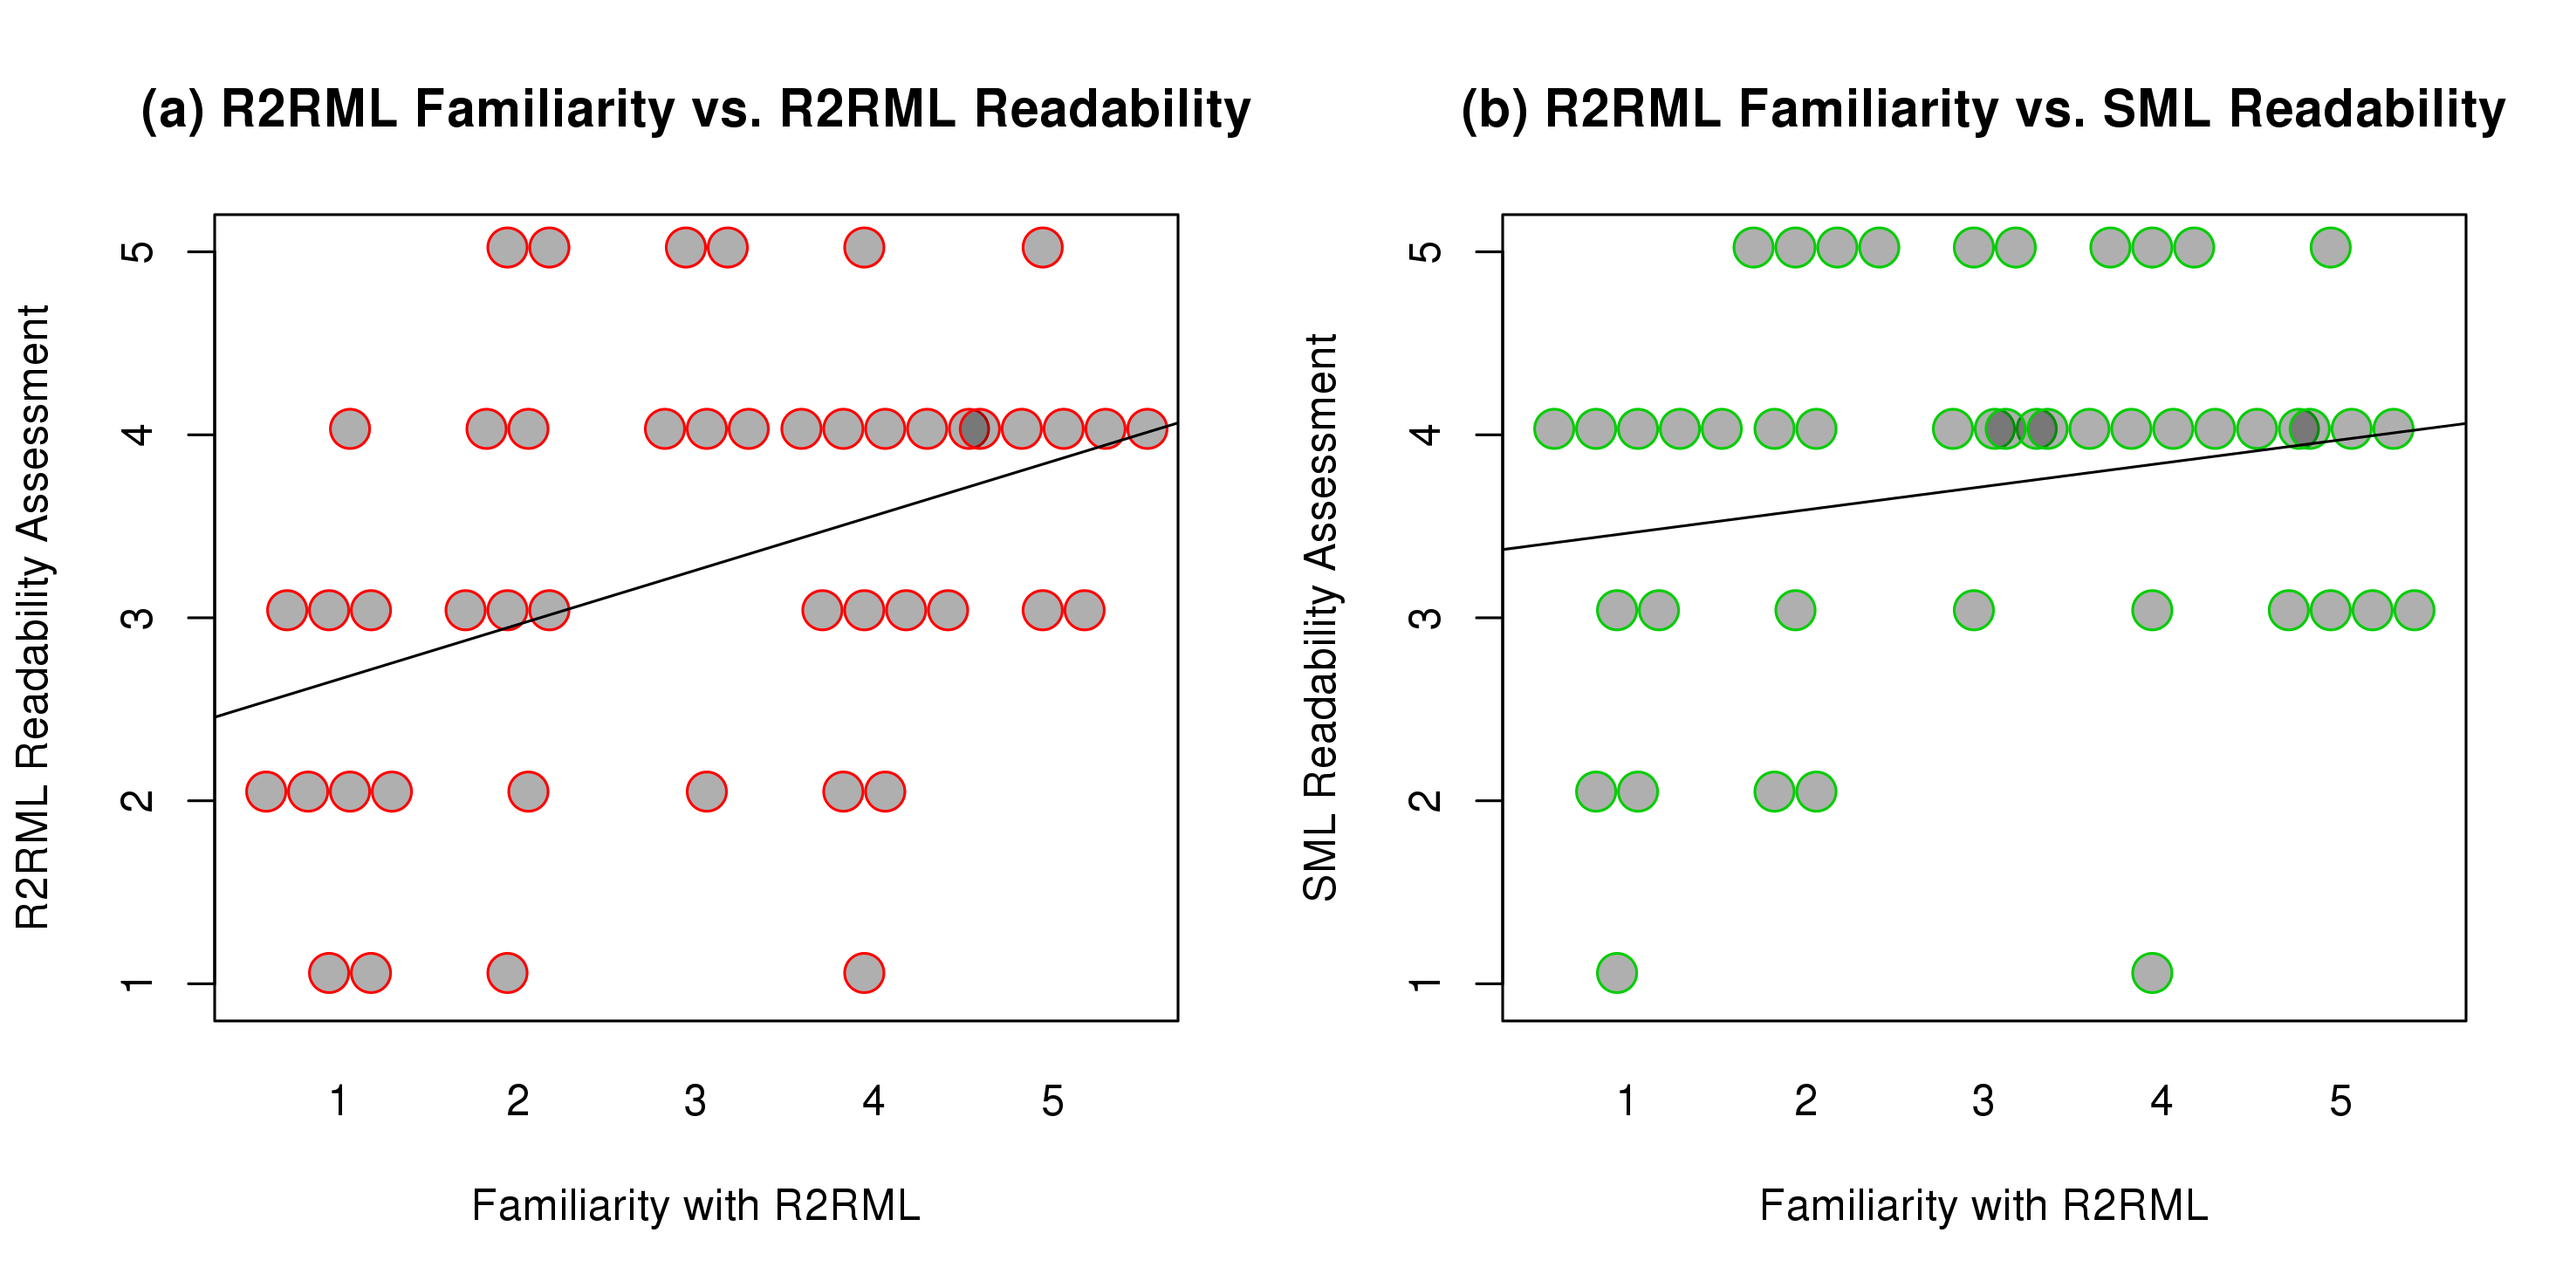
\includegraphics[width=\textwidth]{pics/fam_vs_read}
%\vspace{-15pt}
 \caption{The plot shows the R2RML familiarity plotted against the readability assessment of R2RML and SML. Overall, SML was judged to be significantly more readable although this effect is reduced for participants already familiar with R2RML.}
 \label{fig:fam_vs_read}
\end{figure*}


\begin{figure*}[!t]
%\begin{subfigure}[c]{0.5\textwidth}
%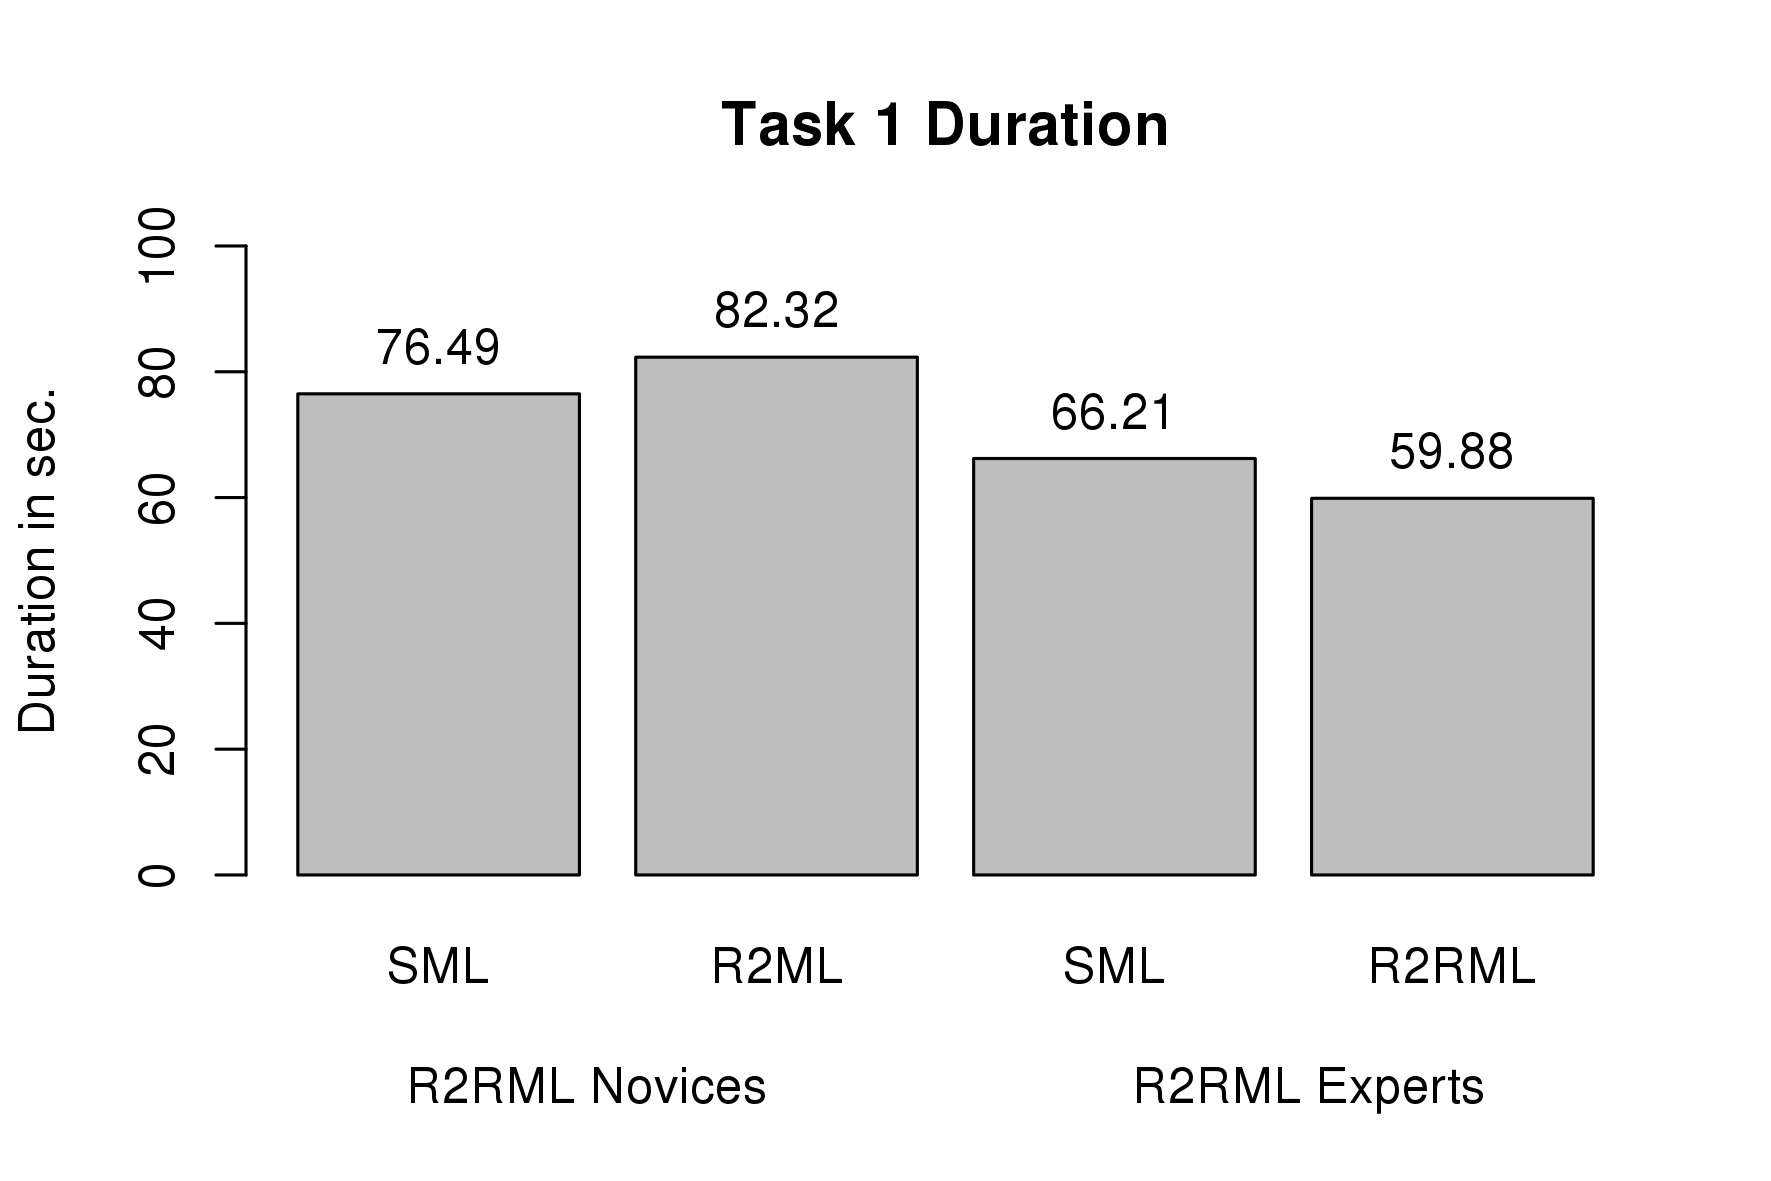
\includegraphics[width=0.99\textwidth]{pics/task1_duration}
%\subcaption{xy}
%\end{subfigure}%
%\begin{subfigure}[c]{0.5\textwidth}
%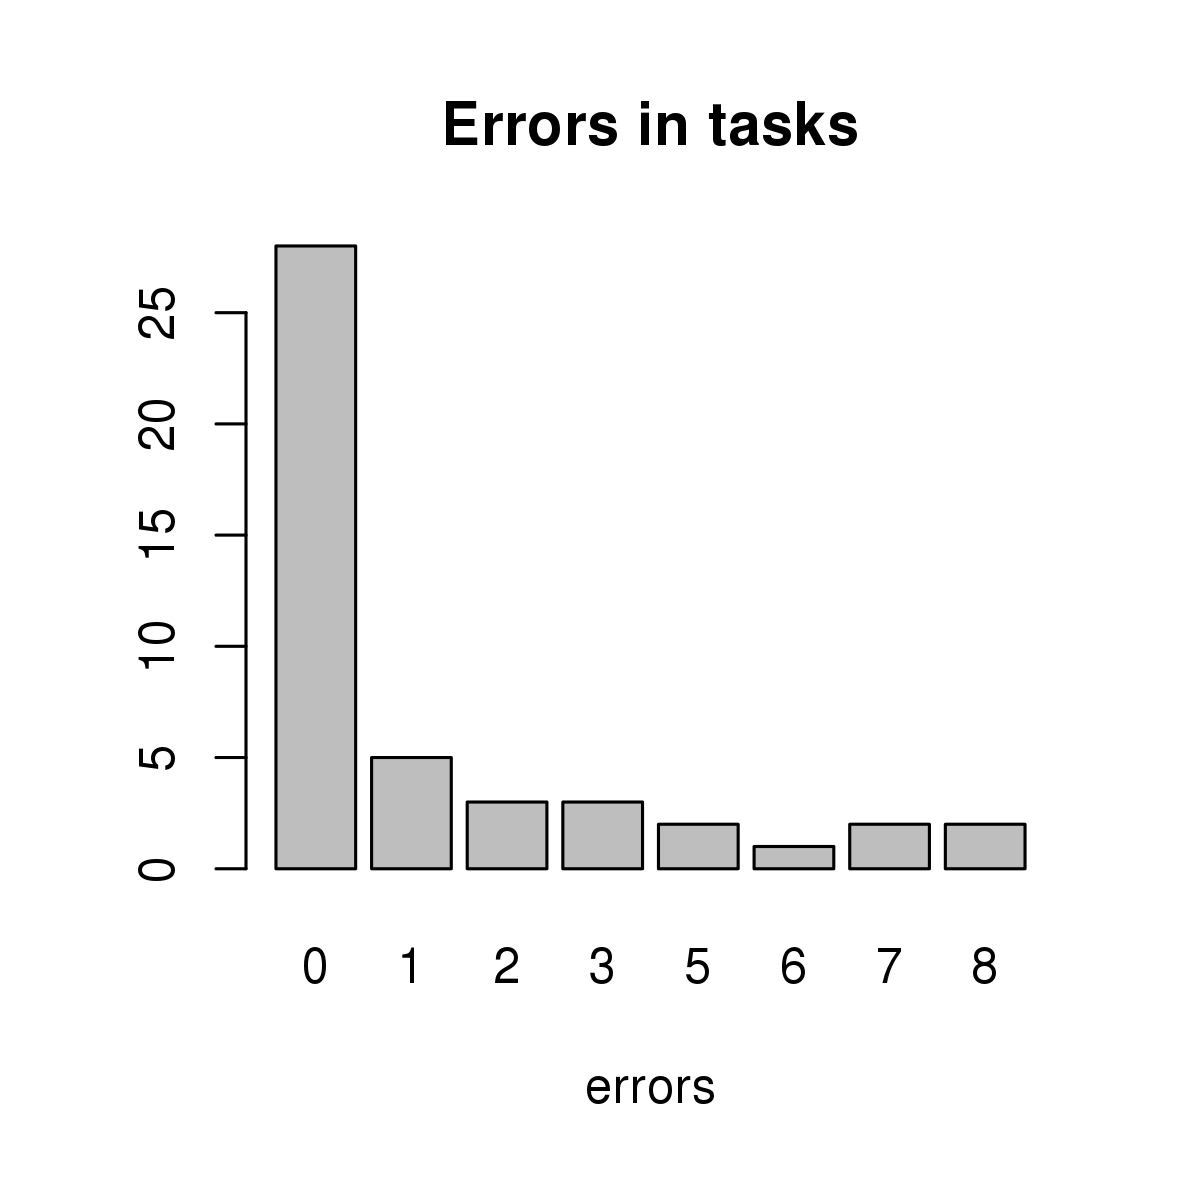
\includegraphics[width=0.99\textwidth]{pics/errors_in_tasks}
%\subcaption{xy}
%\end{subfigure}
%\begin{subfigure}[c]{0.5\textwidth}
%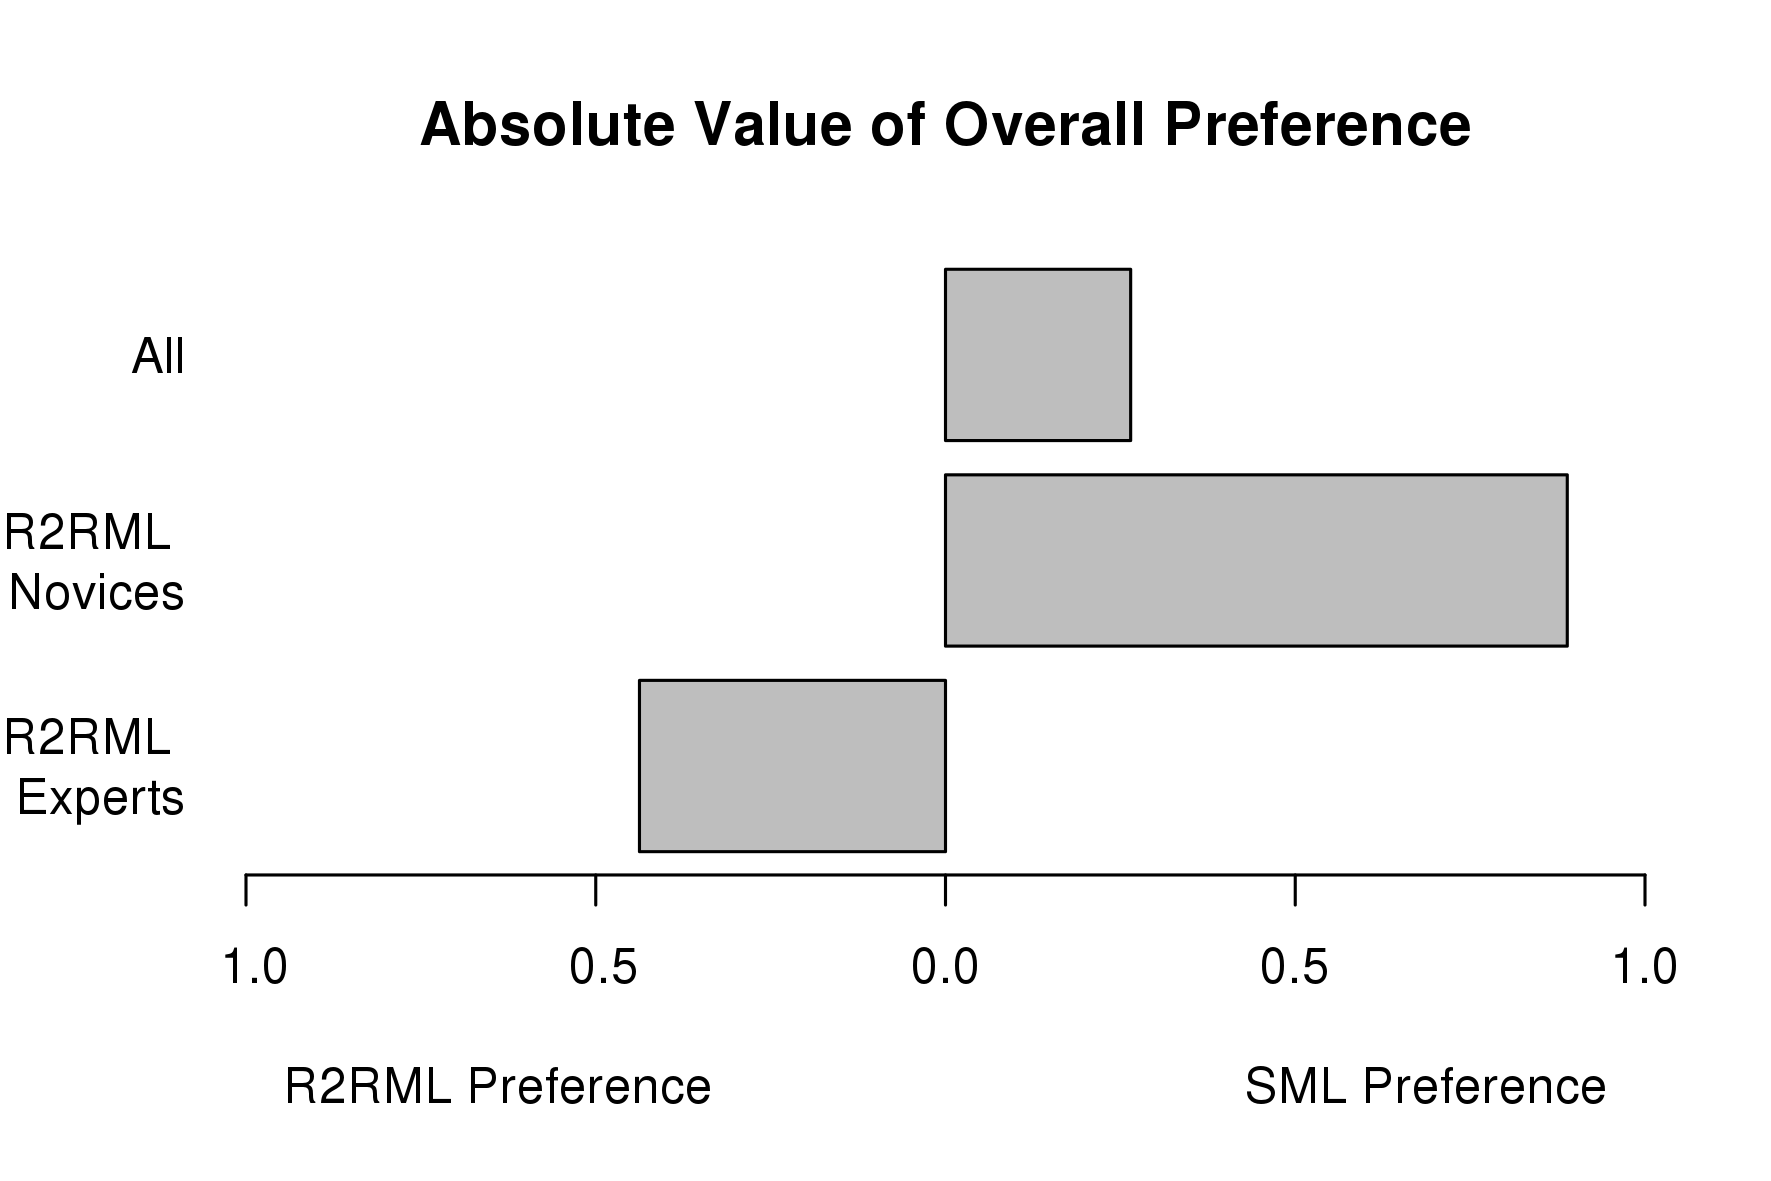
\includegraphics[width=0.99\textwidth]{pics/preference_exp_novice}
%\subcaption{xy}
%\end{subfigure}
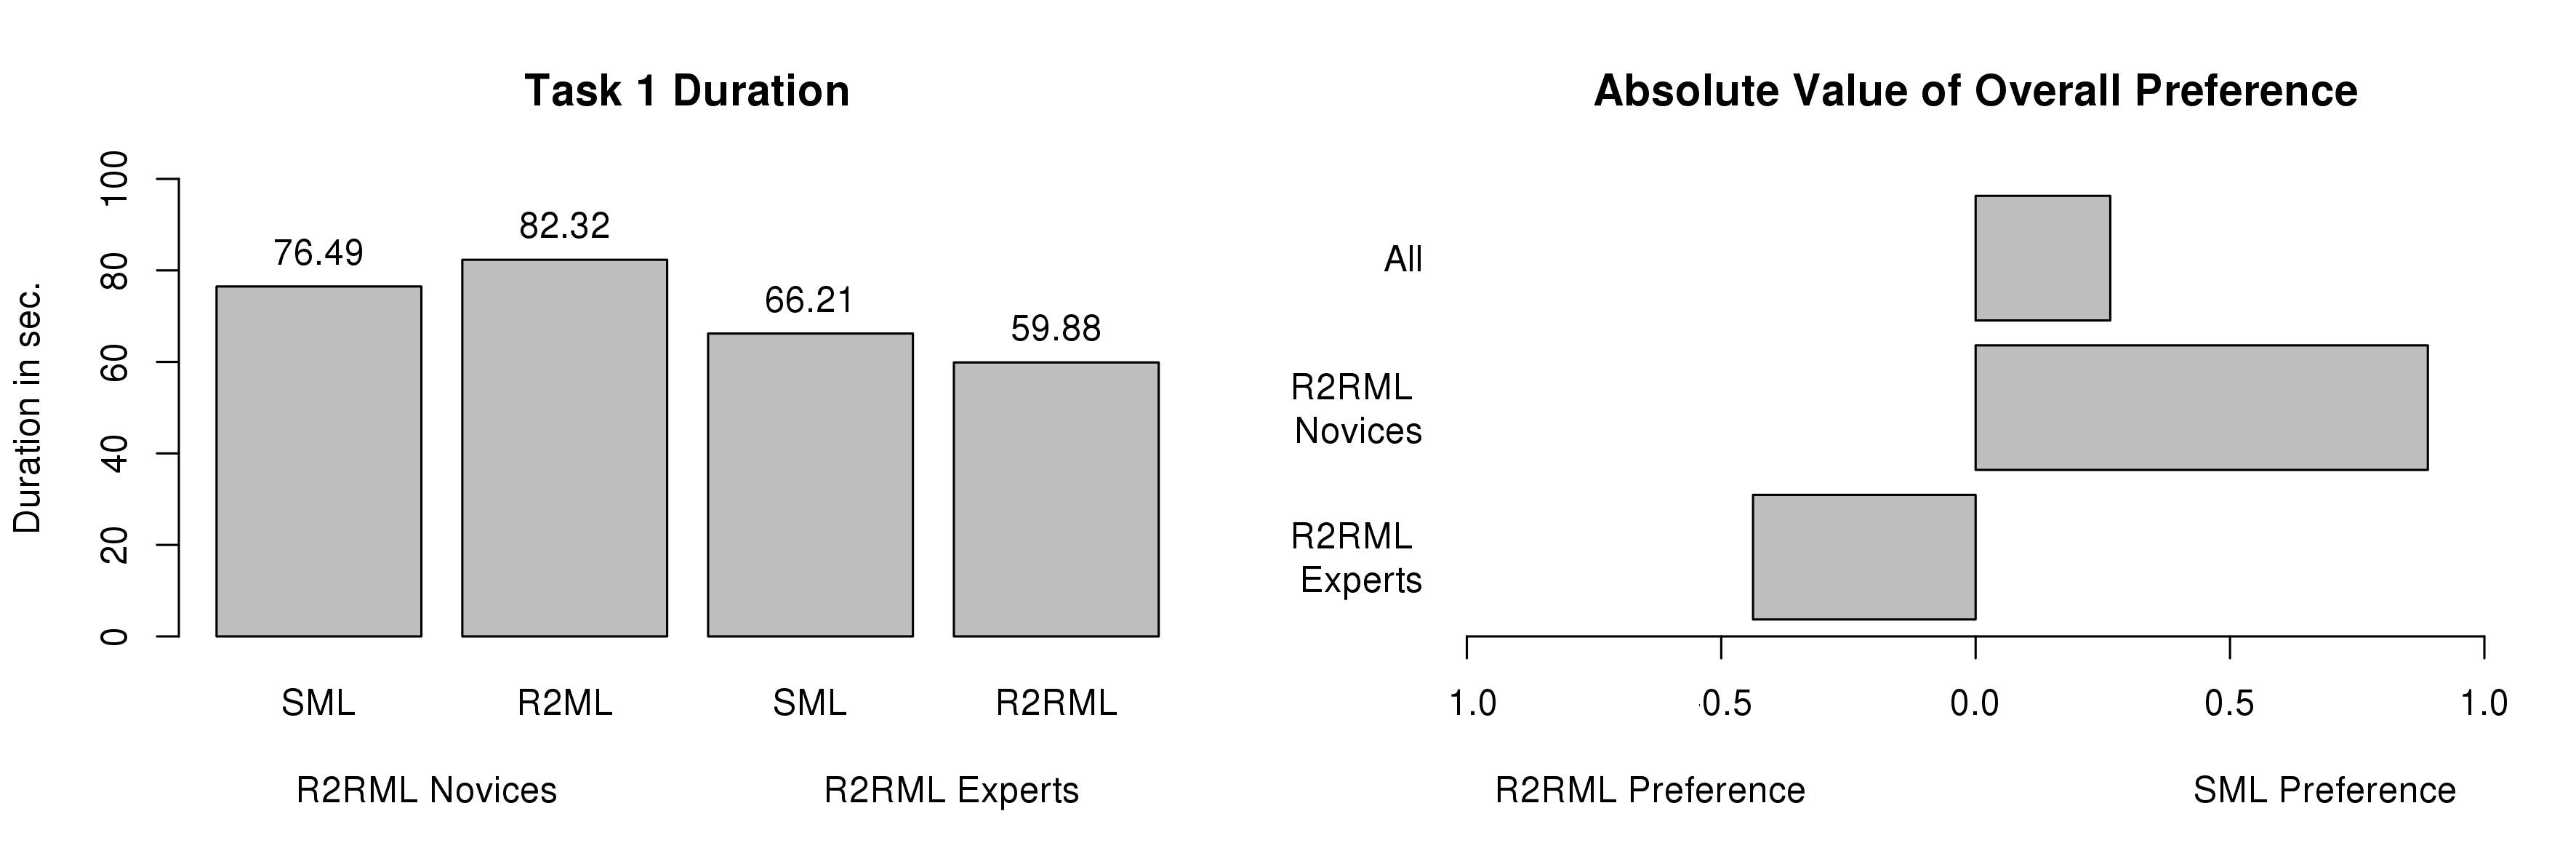
\includegraphics[width=\textwidth]{pics/time_n_pref}
%\vspace{-15pt}
\caption{The figure on the left assesses the time needed to solve an RDB2RDF mapping task. The figure on the right shows the preference for a mapping language. Overall, SML tasks required less time and the language was preferred, although this does not hold when considering only R2RML experts.}
\label{fig:time_n_pref}
\end{figure*}


We evaluated the SML mapping language to clarify the following questions:

\begin{compactenum}
 \item Is SML easier to read than R2RML and does SML have a lower entry barrier than R2RML?
 \item Can people understand SML mappings or R2RML mappings faster?
 \item If given the choice, would people prefer SML or R2RML?
\end{compactenum}

\subsection{Experimental Setup}

We set up a survey, which consists of three parts:

\begin{compactenum}
 \item Questions about prior expertise of the participant.
 \item Test questions for SML and R2RML.
 \item An assessment of the characteristics of SML and R2RML by the participants.
\end{compactenum}

We used a standard star rating for most questions ranging from 1 star (lowest value) to 5 starts (highest value).
The comparison with R2RML was performed as it is the current W3C standard for RDB2RDF mapping.

In the fist part, we asked participants to state their familiarity with the SML and R2RML languages as well as with related concepts such as the Turtle syntax and the SQL and SPARQL query languages.
In the second part, we had 5 different tasks for participants.
Each task was formulated for SML and R2RML with renamed classes and properties.
In the first 3 tasks, participants had to select the subset of 4 shown triples, which was actually generated from a given mapping.
The tasks were ordered by complexity of the mapping specification.
In the 4th and 5th task, the inverse needed to be performed:
Given a target RDF output, participants had to select those mappings from 4 presented mappings, which generates the target output.
Finally, in the third part of the survey, participants had to assess a) the difficulty of the presented tasks, b) whether they could make sense of the SML and R2RML mappings, c) whether they found SML and R2RML easy to read, d) whether they would consider using SML for RDB2RDF tasks and e) whether they have a preference between SML and R2RML.

The survey was distributed to the Semantic Web and Linked Data mailing lists and announced on Twitter.

\subsection{Results}
%\vspace{-5mm}




Overall, a total of 102 participants took part in the survey, of which 73 completed the survey.
We removed entries with an completion time below 500 seconds in order to remove bot entries and carefully assessed the removed entries.
46 participants remained out of which 28 answered all test questions correctly.
The 46 participants required an average time of 1243.1 seconds to complete the survey.
As a result, the overall time valid participants spent on the survey was 953 minutes.
All results of the survey can also be directly obtained and analysed at the SML project website.

The averaged results of the survey are shown in Table~\ref{tab:eval_overview}.
The self assessment scores in Table~\ref{tab:eval_overview} illustrate that the audience is interested in RDB2RDF conversions and that the participants are familiar with Turtle (TTL), SPARQL and SQL.
R2RML familiarity is considerably lower with an average of 3 and SML relatively unknown (1.74).

We discuss each of our evaluation questions in turn:

\emph{Readability and Entry barrier:} Figure~\ref{fig:fam_vs_read} shows that SML appears to have a lower entry barrier than R2RML.
Participants who were familiar with R2RML already judged both languages to have similar readability.
However, participants who were less familiar with R2RML judged SML to be much more readable than R2RML and gave high readability scores.

\emph{Time needed to solve tasks:}
For this task, we randomly started the survey either with either an SML or R2RML task to be able to assess this evaluation question.
The median time required for completing completing in R2RML was 67.08 seconds and for SML 69.23 seconds, giving R2RML a slight edge.
In a more thorough analysis, Figure~\ref{fig:time_n_pref} shows the time required to solve the first RDB2RDF mapping task in the survey, for R2RML experts (self assessment greater or equal 4) and R2RML novices (self assessment less 4).
R2RML experts require less time for solving the task in the R2RML, however R2RML novices appear are able to complete the task faster using SML.
It is further clear that R2RML experts require less time for solving the task regardless of the utilized language.
It should be noted that there is an unknown amount of time required to understand the task irrespective of the mapping language, i.e.~the difference between the mapping language is larger than depicted.


\emph{Overall preference:} Figure~\ref{fig:time_n_pref} shows that there is an overall preference for SML. This preference does not hold when considering only the group of R2RML experts, but is very significant when considering people not familiar with any of the two mapping languages.


\section{Conclusions and Future Work} %no future work so far (not strictly needed) %  and Future Work} \todo{[Claus,Jens]}
\label{sec:conclusion}
%\vspace{-5mm}
In this article, we presented work towards a unified model for RDB2RDF mappings and the
lightweight mapping language \emph{SML} that reuses familiar elements of SPARQL
and SQL in order to lower the learning curve and ease the manual writing and maintenance of view definitions.
An extensive public survey confirmed that this is the case.
%\todo{R3: would need to be supported with a usability study}
We provided an in-depth comparison of how SML relates to the R2RML standard, and
detailed how the former can be automatically converted to the latter.
%A comprehensive formalization of the RDB-RDF rewriting process based the
%definition of RDF views of a relational database and bindings, which bridge
%between the relational and SPARQL algebra.

SML has been successfully deployed in several scenarios:
We created SML mappings for the BSBM and SP2 benchmarks, two
popular SPARQL benchmarks that are often used for evaluating RDB2RDF
mappers.
Most prominently, we created SML mappings for transforming the
OpenStreetMap (OSM) database to RDF. These efforts are carried out
as part of the LinkedGeoData\footnote{\url{http://linkedgeodata.org/}} (LGD) project,
where we give access to more than 25 billion OSM RDF triples created through
SPARQL-to-SQL rewriting over about 3 billion relational rows via more than 40
SML view definitions.

%LGD also includes mappings for the GADM dataset
Furthermore, SML mappings have been created for two large scale
linguistic resources: One is the mapping of the Wortschatz
database\footnote{\url{http://www.wortschatz.uni-leipzig.de/}}, which contains
statistics, such as frequency and co-occurrences, about words in more
than 240 languages.
The other resource is PanLex\footnote{\url{http://ld.panlex.org}}, which is
a database holding translations of about 19 million expression extracted from
over 2.000 sources. Links to the corresponding SML mappings are published
together with our other SML related
resources\footnote{\url{http://sml.aksw.org}}.

In general, we believe that mapping relational structures to RDF will stay a highly important topic in research and practice to provide an unobtrusive transition towards the use of semantic technologies.
Providing engineers an intuitive yet powerful language is a crucial step to ease this transition.
Future work will continue on extending the formalizations as well as sorting out details based on community feedb,
such as whether an explicit \texttt{FROM QUERY} syntax for specifying SQL queries is preferred over
the current approach where this is implied by the use of triple quotes.

%\todo{R2: The weakness of SML also should be discussed}
%\url{http://sml.aksw.org}.
%Todo factor out the sml parser
%This work is the first step in a larger research agenda:
%In the future, we aim to remove even more barriers between the relational and
%RDF worlds.
%Currently, our mapping approach one-directional and read-only: queries are
% translated from SPARQL to SQL and query results from SQL to SPARQL.
%In the future, we plan to make the RDB-RDF mapping writable by enabling SPARQL
% updates, which are translated into updates of the underlying relational database.
%An interesting research direction, for which our formalization could be
% exploited, are bi-directional and hybrid mapping allowing an RDBMS to access RDF data and a possible incorporation of relational and RDF sources in a single mapping.
%A further research question is how inferencing and reasoning features can be
% integrated into the RDB-RDF mapping and rewriting.
%Another issue in this regard is how the SPARQL 1.1
% features\footnote{\url{http://w3.org/TR/sparql11-query/}}, such as property paths of arbitrary length, can be efficiently supported in the SPARQL-SQL rewriting.
%Furthermore, although we believe that SML is easier to use while offering similar functionality and expressiveness as R2RML
%the RDF based mapping language R2RML\footnote{\url{http://w3.org/TR/r2rml/}}, % no need for the full name and URI here after mentioning R2RML a hundred times ;)
%the latter has been standardized very recently and should therefore be supported by the Sparqlify system.
%Yet, we believe that Sparqlify-ML is in most cases easier to learn and use than R2RML, and therefore see future efforts on improving Sparqlify-ML as complementary.


% Jens: I removed the last part as it was just stating that Sparqlify should support R2RML, which is not the point of the article.

%\section*{Acknowledgment}
%\vspace{-5pt}
%This work was supported by grants from the EU's 7th Framework Programme provided for the projects LOD2 (GA no. 257943) and GeoKnow (GA no. 318159).

%\vfill
%\columnbreak

%\bibliographystyle{abbrv}
%\bibliography{../../bib/aksw,literature}



